\documentclass[10pt,a4paper]{article}
\usepackage{sketch} % See researchsketch.sty %
\usepackage{enumitem}
\usepackage[linesnumbered,ruled,vlined]{algorithm2e}
\usepackage{amsmath}
\usepackage{listings}
\usepackage{array}
\usepackage{tikz}
\usepackage{graphicx}
\usepackage{float}
\renewcommand{\lstlistingname}{\bfseries Program}
\DeclareMathOperator*{\argmin}{arg\,min}
\makeatletter
\def\fnum@lstlisting{%
  \bfseries\lstlistingname
  \ifx\lst@@caption\@empty\else~\thelstlisting\normalfont\fi}%
\makeatother
\lstdefinestyle{myStyle}{
    belowcaptionskip=1\baselineskip,
    breaklines=true,
    frame=none,
    numbersep=5pt, 
    basicstyle=\footnotesize\ttfamily,
    keywordstyle=\bfseries\color{green!40!black},
    commentstyle=\bfseries\color{purple!60!black},
    identifierstyle=\color{blue},
}
\setenumerate[1]{itemsep=0pt, partopsep=5pt,topsep=5pt}
\setitemize[1]{itemsep=0pt, partopsep=5pt,topsep=5pt}
\author{1155189917}
\title{Research Note}
\pagestyle{fancy}
\renewcommand{\headrulewidth}{0pt}
\fancyhf{}
\rfoot{Page \thepage}
\date{\today}
\begin{document}
\noindent Convergence of \texttt{ASkewSGD}: A Quantization-Aware-Training Algorithm for Deep Neural Networks\\
Student: WONG, Hok Fong\hfill Research Progress Overview (Summer 2025)\\
\phantom{}\hrulefill
\setlength{\parindent}{0pt}
\setlength{\parskip}{5pt}
\section{Background} \marginpar{\small\textsf{\mbox{Jan 9, 2025}}}

We are interested in solving the optimization problem related to learning a quantized neural network (QNN),
\[\min_{\mathbf{w}\in\mathcal{Q}} \ell(\mathbf{w})\text{, where }\ell(\mathbf{w})=\mathbb{E}_{(\mathbf{x},y)\sim p_{\text{data}}} [\ell(f(\mathbf{x},\mathbf{w}), y)],\]
where $\ell:\mathbb{R}^d\to \mathbb{R}$ denotes the training loss, $\mathcal{Q}\subset \mathbb{R}^d$ is the set of quantization levels,
$d$ is the number of parameters in the neural network, $p_{\text{data}}$ is the training distribution \ref{1}.

We do not necessarily aim to solve the above (hard, combinational) optimization problem globally and optimally.
Instead, we want to find discrete weights $\mathbf{w}\in \mathcal{Q}$ that remain satisfactory when compared to the
non-quantized continuous weights \ref{2}.

\textbf{Goal.} Given a reasonably smooth function $\ell$, develop an algorithm with certain guarantees that converges
to a close-by quantized weight of a locally, or globally, optimal continuous weight with similar performance.

We turn to consider the smoothed sequence of interval-constrained optimization problems ($\mathcal{P}_\varepsilon$),
\[\min_{\mathbf{w}\in C_\varepsilon} \ell(\mathbf{w}), C_\varepsilon=\{\mathbf{w}\in \mathbb{R}^d: g_\varepsilon(\mathbf{w})\geq 0\},\]
where $\varepsilon$ is an annealing parameter that converges to zero.

Previously, Muehlebach and Jordan \ref{3} reformulated the position constraints into forward ``velocity'' constraints by considering a
linear and convex approximation of the original feasible set with the objective function satisfying the Mangasarian-Fromovitz condition.

\textbf{Definition (Mangasarian-Fromovitz Constraint Qualification).} $\forall \mathbf{x}\in \mathbb{R}^d$, $\exists \mathbf{w}\in \mathbb{R}^n$
s.t. $\nabla g_i(\mathbf{x})^\top \mathbf{w}>0$ for all $i\in I(\mathbf{x})$, where $I(\mathbf{x})=\{i\in \mathbb{Z}\bigm| g_i(\mathbf{x})\leq 0\}$.

By MFCQ, the set $V_\alpha(\mathbf{w})$, $V_\alpha(\mathbf{w})=\{\mathbf{v}\in\mathbb{R}^d: \nabla g_i(\mathbf{w})^\top \mathbf{v}\geq -\alpha g_i(\mathbf{w})\}$, is considered as an extension of the tangent cone outside of the feasible set, and is always a convex polyhedron.

\begin{algorithm}[H]
  \caption{Muehlebach-Jordan Algorithm}
  \For{$k=1,2,\ldots$}{
    $\mathbf{v}^{(k)} = \arg\min_{\mathbf{v}\in V_\alpha(\mathbf{w}^{(k)})} (1/2)\lVert \mathbf{v}+\nabla \ell(\mathbf{w}^{(k)})\rVert^2$.

    $\mathbf{w}^{(k+1)}=\mathbf{w}^{(k)}+\gamma_k \mathbf{v}^{(k)}$.
  }
\end{algorithm}


We note that $\alpha$ controls the trade-off betweeen two objectives: for large $\alpha$, the emphasis is on the convergence to the feasible set,
while for small $\alpha$, the focus is on reducing the objective function \ref{3}.

Muehlebach and Jordan's algorithm \ref{3} is then extended by Leconte et al. \ref{1} to the quantization-aware training algorithm \texttt{ASkewSGD}.

\textbf{Definition (Remoteness Measurement of the Quantization Set).} Let $\varepsilon\in[0,1]$, $w_i\in \mathcal{Q}_i, i\in [d]$,
where $\mathcal{Q}_i=\{q^{(1)}_i, \ldots, q^{(K_i)}_i\}$ are sets of quantization values defined coordinate-wise. We define the piecewise function
\begin{align*}\psi_{i}(w_i;\varepsilon):=\begin{cases}\varepsilon-(q_i^{(1)}-w_i)^2                    & w_i < q_i^{(1)},                                \\
             \varepsilon-(w_i-q_i^{(j-1)})^2(w_i-q_i^{(j)})^2 & q_i^{(j-1)}\leq w_i < q_i^{(j)}, j=2,\ldots, K, \\
             \varepsilon-(w_i-q_i^{(K_i)})^2                  & w_i \geq q_i^{(K_i)},\end{cases}
\end{align*} for all $w_i\in\mathbb{R}$ and $i\in [n]$.

We impose constraints on each parameter of the neural network, by setting $g_i(\mathbf{w})=\psi_i(w_i;\varepsilon)$. This then forms the feasible
set $C_\varepsilon$. Furthermore, $V_{\varepsilon, \alpha}=\{\mathbf{v}\in\mathbb{R}^d: v_i \psi'_i (w_i;\varepsilon)\geq -\alpha \psi_i(w_i;\varepsilon) \text{ for } i\in I_\varepsilon(\mathbf{w})\}$, where $I_\varepsilon(\mathbf{w})=\{i\in[d]: \psi_i(w_i;\varepsilon)\leq 0\}$, the normal cone of $C_\varepsilon$ is given by $N_{C_\varepsilon}=\{-\sum_{i\in I_\varepsilon(\mathbf{w})} \lambda_i\nabla g_i(\mathbf{w}), \lambda_i\in \mathbb{R}_+ \}$.

\begin{algorithm}[H]
  \caption{\texttt{ASkewSGD} Algorithm for QNN Training}
  \For{$k=1,2,\ldots$}{
    Obtain a stochastic gradient $\widehat{\nabla\ell}(\mathbf{w}^{(k)})$.

    $\widehat{\mathbf{v}}^{(k)} = \arg\min_{\mathbf{v}\in V_{\varepsilon,\alpha}(\mathbf{w}^k)} (1/2)\lVert \mathbf{v}+\widehat{\nabla \ell}(\mathbf{w}^{(k)})\rVert^2$.

    $\mathbf{w}^{(k+1)}=\mathbf{w}^{(k)}+\gamma_k \widehat{\mathbf{v}}^{(k)}$.
  }
\end{algorithm}

The optimization problem \[\argmin_{\mathbf{v}\in V_{\varepsilon, \alpha}(\mathbf{w})} (1/2) \lVert \mathbf{v}+\mathbf{u}\rVert^2\] has an explicit solution:
\begin{align*}[\mathbf{s}_{\varepsilon, \alpha}(\mathbf{g},\mathbf{w})]_i:=\begin{cases}-g_i                                                    & \text{if }\psi_i(w_i;\varepsilon)>0 \text{ or }-g_i\cdot \psi_i'(w_i;\varepsilon)\geq -\alpha \psi_i(w_i;\varepsilon)\geq 0, \\
             \text{clip}(-\alpha\psi_i(w_i;\varepsilon)/\psi'_i(w_i;\varepsilon), M_c) & \text{otherwise}.\end{cases}
\end{align*}

Furthermore, the set of stationary points are given by the Karush-Kuhn-Tucker condition:
\[\mathcal{Z}_\varepsilon:=\{\mathbf{w}\in C_\varepsilon: \mathbf{0}\in -\nabla \ell(\mathbf{w})-N_{C_\varepsilon}(\mathbf{w})\}.\]

That is, $\mathbf{w}\in \mathcal{Z}_\varepsilon$ if and only if $[\nabla\ell(\mathbf{w})]_i=0$ when $\psi_i(w_i;\varepsilon)> 0$ and $\text{sign}([\nabla\ell(\mathbf{w})]_i)=\text{sign}(\psi_i'(w_i;\varepsilon))$ when $\psi_i(w_i;\varepsilon)= 0$.

\section{Existing Results} \marginpar{\small\textsf{\mbox{Jan 10, 2025}}}

To set up the analysis, we list the following conditions on the loss function and the step sizes.

\textbf{Assumption 1.} The function $\ell$ is continuously differentiable and $M_\ell$-smooth, i.e. \[\lVert \nabla\ell(\mathbf{x})-\nabla \ell(\mathbf{y})\rVert^2\leq M_\ell \lVert \mathbf{x}-\mathbf{y}\rVert^2\text{ for any }\mathbf{x}, \mathbf{y}\in\mathbb{R}^d.\]

\textbf{Assumption 2.} The function $\ell$ is $d$-times continuously differentiable.

\textbf{Assumption 3.} The stepsizes $(\gamma_k)_{k\geq 0}$ are positive, non-summable and square-summable, i.e. \[\sum\limits_{k=0}^\infty \gamma_k=\infty, \sum\limits_{k=0}^\infty \gamma_k^2<\infty.\]

\textbf{Assumption 4.} The function $\ell$ is continuously differentiable and $L_\ell$-Lipschitz continuous, i.e. \[| \ell(\mathbf{x})- \ell(\mathbf{y})|^2\leq L_\ell \lVert \mathbf{x}-\mathbf{y}\rVert^2\text{ for any }\mathbf{x}, \mathbf{y}\in\mathbb{R}^d.\]

\textbf{Lemma 1.} (Leconte et al., \ref{1}) Under A3 and A4, it holds that $\lim\sup_{k\to\infty} \text{d}(\mathbf{w}^{(k)}, C_\varepsilon)=0$ almost surely.

\textit{Proof.} See Leconte et al. \ref{1}, an asymptotic result.

\textbf{Theorem 1. (Asymptotic Convergence Guarantees with Lipschitz Continuity)} (Leconte et al., \ref{1}) Assume A2, A3, A4 and $0<\varepsilon\leq \inf_{1\leq i\leq d}\inf_{1\leq j< K_i} \lvert q^{(j)}_i - q^{(j+1)}_i\rvert^4/16$ holds, where $\{q^{(j)}_i\}$ are the quantization levels, $\ell(\mathbf{w}^{(k)})$ converges and $\lim_{k\to\infty} \text{d}(\mathbf{w}^{(k)}, \mathcal{Z}_\varepsilon)=0$ almost surely.

\textbf{Remark.} We try to remove A2, A4. We also attempt to investigate the general behavior of \texttt{ASkewSGD} without A3.


% Denote $M_1=\max\{M_{c}, L_\ell\}$. Now, for all $i\in [n]$, we have $\lVert \widehat{\nabla}\ell(\mathbf{w}^{(k)})\rVert_2\leq M_1$ and $\lvert v^{(k)}_i\rvert\leq M_1$, and thus $\lvert w^{(k+1)}_i-w^{(k)}_i\rvert \leq \gamma_k M_1$.

% Three crucial steps for the correctness of this lemma will then be introduced. The three steps involved will correspond to Claims 1-3, Claims 4-5, and Claims 7-8.

% \textit{Claim 1.} For $i\in \{1,2, \ldots ,d\}$, and for $2\leq j\leq K_i-1$ if the set $\left[(q_i^{(j)}+q_i^{(j-1)})/2, (q_i^{(j)}+q_i^{(j+1)})/2\right)$ is visited by $w_i^{(k)}$ infinitely often, then there is $k_0$ such that for all $k>k_0$, $w_i^{(k)}\in \left[(q_i^{(j)}+q_i^{(j-1)})/2, (q_i^{(j)}+q_i^{(j+1)})/2\right)$.

% Fix a $j$ and denote $[q_-, q_+]$ the set $C_{\varepsilon,i}\cap\left[(q_i^{(j)}+q_i^{(j-1)})/2, (q_i^{(j)}+q_i^{(j+1)})/2\right)$, where $C_{\varepsilon,i}$ is the projection of $C_\varepsilon$ on the $i$-th coordinate.
% Define $$k_0=\sup\{k: \gamma_k M_1\geq \max(q_--(q_j^i+q_{j-1}^i)/2, (q_j^i+q_{j+1}^i)/2-q_+)\}.$$ Consider $k \geq k_0$, suppose $(q_i^{(j)}+q_i^{(j-1)})/2\leq w_i^{(k)} < q_-$ (the left side of the interval), then the $\mathbf{w}^{(k)}$ is pushed to the right and $w_i^{(k)}\leq w_i^{(k+1)}$.

% Furthermore, by definition of $k_0$, it holds that $w_i^{(k+1)}\leq q_-+\gamma_k M_1\leq (q_i^{(j)}+q^{(j+1)}_i)/2$.
% This implies that, in this case $w_i^{(k+1)}$ stays in $[(q_i^{(j)}+q_i^{(j-1)})/2, (q_i^{(j)}+q_i^{(j+1)})/2)$.

% Otherwise, suppose $q_+\leq w_i^{(k+1)} < (q_i^{(j)}+q^{(j+1)}_i)/2)$ (the right side of the interval), then the $\mathbf{w}^{(k)}$ is pushed to the left and $w_i^{(k)}\geq w_i^{(k+1)}\geq q_+ - \gamma_k M_1\geq (q^{j}_i+q^{(j-1)}_i)/2$. Finally, if $w_i^{(k)}\in [q_-, q_+]$, then by the definition of $k_0$, we obtain $w_i^{(k+1)}\in [(q^{(j)}_i+q^{(j-1)}_i)/2, (q_i^{(j)}+q^{(j+1)}_i)/2)$.

% Thus, we have shown that for $k\geq k_0$ if $w^{(k)}_i$ stays within the interval $[(q^{(j)}_i+q^{(j-1)}_i)/2, (q^{(j)}_i+q^{(j+1)}_i)/2)$, then for all $k'\geq k$, $w^{(k')}_i\in [(q_i^{(j)}+q_i^{(j-1)})/2, (q_i^{(j)}+q_i^{(j+1)})/2)$.

% Similarly, we can prove the two statements below corresponding to the edge cases.

% \textit{Claim 2.} For $i\in \{1,2, \ldots ,d\}$, if the set $(-\infty, (q_i^{(1)}+q_i^{(2)})/2)$ is visited by $w^{(k)}_i$ infinitely often, then there is $k_0$ such that for all $k>k_0$, $w^{(k)}_i\in (-\infty, (q^{(1)}_i+q^{(2)}_i)/2)$.

% \textit{Claim 3.} For $i\in \{1,2, \ldots ,d\}$, if the set $[(q^{(K_i-1)}_i+q^{(K_i)}_i)/2, +\infty)$ is visited by $w^{(k)}_i$ infinitely often, then there is $k_0$ such that for all $k>k_0$, $w^{(k)}_i\in [(q^{(K_i-1)}_i+q^{(K_i)}_i)/2, +\infty)$.

% We can then leave our attention to one of the three intervals $[(q^{(j)}_i+q^{(j-1)}_i)/2, (q^{(j)}_i+q^{(j+1)}_i)/2), (-\infty, (q^{(1)}_i+q^{(2)}_i)$, or $[(q^{(K_i-1)}_i+q^{(K_i)}_i)/2, +\infty)$.

% \textit{Claim 4.} There is $k_1\geq k_0$, such that if there are two indices $m_+\geq m_->k_0$ such that $w^{(m_-)}_i<q_-<q_+<w^{(m_+)}_i$, then there is $m$, satisfying $m_-\leq m \leq m_+$, such that $w^{((m))}_i\in [q_-, q_+]$.

% Define $k_1=\sup\{k:\gamma_k M_1\geq q_+-q_-\}$.
% Let $m_-, m_+$ be given and consider $m=\inf\{k\geq m_-: w^{(k)}_i\geq q_-\}$. It holds that $w^{(m-1)}_i<q_-\leq w^{(m)}_i\leq w^{(m-1)}_i+\gamma_k M_1$.

% Since $m\geq k_1$, this implies that $w^{(m)}_i \leq q_-+\gamma_k M_1\leq q_+$, which proves the claim.

% \textit{Claim 5.} There is $k_1\geq k_0$, such that if there are two indices $m_-\geq m_+>k_0$ such that $w_{m_-}<q_-<q_+<w_{m_+}$, then there is $m$, satisfying $m_+\leq m \leq m_-$, such that $w_m^i\in [q_-, q_+]$ .

% The proof of Claim 5 is similar to Claim 4. Claims 4, and 5 show that there are only three behaviors of $w^{(k)}_i$. These three conditions will be treated by Claims 6, 7, and 8, respectively.

% \textit{Claim 6.} Let $k\geq k_0$. If $w^{(k)}_i$ visits $[q_-, q_+]$ infinitely often, then $\lim \sup_{k\to\infty} w^{(k)}_i\leq q_+$ and $\lim\sup_{k\to\infty} w^{(k)}_i\geq q_-$.

% We first show the case of $\lim \sup_{k\to\infty} w^{(k)}_i\leq q_+$.

% Suppose that $w^{(k)}_i>q_+$, then $w^{(k+1)}_i\leq w^{(k)}_i$, and otherwise if $w^{(k)}_i\leq q_+$ then $w^{(k+1)}_i\leq q_++\gamma_k M_1$.

% We note that $\gamma_k$ is non-increasing and thus no $w^{(k')}$ where $k'\geq k$ can go further than $q_++\gamma_k M$ since it immediately receives the skewing force after the constraint violation.

% Tending $k$ to infinity yields $\lim \sup_{k\to\infty} w_k^i\leq c_+$. It is easy to see that the other case also holds.

% \textit{Claim 7.} If for all $k\geq k_0$ large enough, $w^{(k)}_i>q_+$, then $w^{(k)}_i\to q_+$.

% For all $k$ large enough, the sequence $w^{(k)}_i$ is decreasing. From the given condition that $w^{(k)}_i>q_+$, the sequence has a limit. 

% Assume the contrary that $\lim_{k\to\infty}w^{(k)}_i\neq q_+$. It holds that $w^{(k+m+1)}_i\leq w^{(k)}_i-M_+ \sum_{j=0}^m\gamma_{k+j}$, where $M_+=\inf\{\min(M_{\varepsilon, c}, \alpha\lvert \psi_i(w_i;\varepsilon)\rvert/ \psi'_{i}(w_i;\varepsilon)):w_i\in [q_+, (q^{(j)}_i+q^{(j+1)}_i)/2)\}>0$. Since $\sum_{j=0}^{\infty} \gamma_j =+\infty$, we have reached a contradiction. $w^{(k)}_i\to q_+$.

% \textit{Claim 8.} If for all $k\geq k_0$ large enough, $w^{(k)}_i<q_-$, then $w^{(k)}_i\to q_-$.

% It holds that $w^{(k+m+1)}_i\geq w^{(k)}_i+M_- \sum_{j=0}^m\gamma_{k+j}$, where $M_-=\inf\{\min(M_{\varepsilon, c}, \alpha\lvert \psi_i(w_i;\varepsilon)\rvert/ \psi'_{i}(w_i;\varepsilon)):w\in ((q^{(j)}_i+q^{(j-1)}_i)/2, q_-]\}>0$. Similar to Claim 7, it is impossible that $\lim_{k\to\infty}w^{(k)}_i\neq q_-$.\qed

\newpage
\section{Current Work} \marginpar{\small\textsf{\mbox{Jan 10, 2025}}}

% \textbf{Targeted Theorem.} (Our work) Assume A1, A3, A5, A6, and $0<\varepsilon\leq \inf_{1\leq i\leq d}\inf_{1\leq j< K_i} \lvert q^{(j)}_i - q^{(j+1)}_i\rvert^2/4$, where $\{q^{(j)}_i\}$ are the quantization levels, $\lim_{k\to\infty} \mathbb{E}[\text{d}(\mathbf{w}^{(k)}, \mathcal{Z}_\varepsilon)]=0$ almost surely.

\textbf{Definition (Quadratic Remoteness Measurement of the Quantization Set).} Let $\varepsilon\in[0,1]$, $w_i\in \mathcal{Q}_i, i\in [d]$,
where $\mathcal{Q}_i=\{q^{(1)}_i, \ldots, q^{(K_i)}_i\}$ are sets of quantization values defined coordinate-wise. We define the piecewise function
\begin{align*}\psi_{i}(w_i;\varepsilon):=\begin{cases}\varepsilon-(q_i^{(1)}-w_i)                  & w_i < q_i^{(1)},                                  \\
             \varepsilon-(q_i^{(j-1)}-w_i)(w_i-q_i^{(j)}) & q_i^{(j-1)}\leq w_i < q_i^{(j)}, j=2,\ldots, K_i, \\
             \varepsilon-(w_i-q_i^{(K_i)})                & w_i \geq q_i^{(K_i)},\end{cases}
\end{align*} for all $w_i\in\mathbb{R}$. This function has a lower order compared to Leconte et al.'s.

\marginpar{\small\textsf{\mbox{May 17, 2025}}}

\textbf{Lemma 2 (Convergence of the Skewing Force).} Under Assumption 4, and fix an arbitrary $0<\varepsilon\leq \inf_{1\leq i\leq d}\inf_{1\leq j<K_i} \lvert q_i^{(j)} - q_{i}^{(j+1)}\rvert^2/4$, where $\{q_i^{(j)}\}$ are the quantization levels. Denote $[q_-, q_+]$ as the set $C_{\varepsilon,i}\cap [(q_i^{(j)}+q_i^{(j-1)})/2, (q_i^{(j)}+q_i^{(j+1)})/2)$, where $C_{\varepsilon,i}$ is the projection of $C_\varepsilon$ on the $i$-th coordinate.
Let $0<\delta_1<(q_i^{(j)}+q_i^{(j+1)}-2q_+)/3$ and $0<\delta_2<(2q_--q_i^{(j)}-q_i^{(j-1)})/3$ be some small perturbations on a quantization level.  Then,
\begin{enumerate}[label=(\alph*)]
  \item \[\left\lvert \frac{-\alpha\psi_i(q_++\delta_1;\varepsilon)}{\psi'_i(q_++\delta_1;\varepsilon)}\right\rvert \leq 2\alpha \delta_1;\]
  \item \[\left\lvert \frac{-\alpha\psi_i(q_--\delta_2;\varepsilon)}{\psi'_i(q_--\delta_2;\varepsilon)}\right\rvert \leq 2\alpha\delta_2.\]
\end{enumerate}
% Moreover, we have $\lim_{k\to\infty} \lVert \mathbf{u}^{(k)}\rVert_2=0$ almost surely.

% \textit{Remark.} We charge the size of the skewing force (denoted by $\mathbf{u}^{(k)}$) on the distance of $\mathbf{w}^{(k)}$ to the feasible set $C_\varepsilon$, $\text{d}(\mathbf{w}^{(k)}, C_\varepsilon)$. Using the $\varepsilon$-$N$ definition of limits, we can pick an arbitrarily small $\delta_1$ such that $\forall k\geq N, \text{d}(\mathbf{w}^{(k)}, C_\varepsilon)\leq \delta_1$. It would be of great use when $\mathbf{w}$ stabilizes and gets close enough to the feasible set - the iterate gets locked in a quantization ``basin''.

\textit{Proof.} By symmetry, we only need to prove the statement as in (a). Note that
  $$\psi_i(q_+;\varepsilon)=\varepsilon-(q_+-q_i^{(j-1)})(q_i^{(j)}-q_+)=0.$$
Also, $$\psi_i'(w;\varepsilon)=2w-q_i^{(j+1)}-q_i^{(j)}.$$


Using (1), we expand the numerator of the left-hand side of (a) and obtain
$$\begin{aligned}
    \psi_i(q_++\delta_1;\varepsilon) & =\varepsilon+(q_++\delta_1-q_i^{(j)})(q_++\delta_1-q_i^{(j+1)})                               \\
                                          & =\varepsilon+(q_+-q_i^{(j)})(q_+-q_i^{(j+1)})+\delta_1(2q_+-q_i^{(j+1)}-q_i^{(j)})+\delta_1^2 \\
                                          & =\delta_1(2q_+-q_i^{(j+1)}-q_i^{(j)})+\delta_1^2<0.
  \end{aligned}$$

Since $\delta_1>0$, we have $\psi_i'(q_++\delta_1;\varepsilon)=2q_++\delta_1-q_i^{(j+1)}-q_i^{(j)}<0$ by (2). Then,
$$\begin{aligned}\left\lvert \frac{-\alpha\psi_i(q_++\delta_1;\varepsilon)}{\psi'_i(q_++\delta_1;\varepsilon)}\right\rvert & =\frac{\alpha\delta_1(2q_+-q_i^{(j)}-q_i^{(j+1)}+\delta_1)}{(2q_+-q_i^{(j)}-q_i^{(j+1)})+2\delta_1} \\
                                                                                                                                   & \leq \frac{\alpha\delta_1(2q_+-q_i^{(j)}-q_i^{(j+1)})}{(2q_+-q_i^{(j)}-q_i^{(j+1)})+2\delta_1}           \\
                                                                                                                                   & =\alpha\delta_1-\frac{\alpha\delta_1^2}{(2q_+-q_i^{(j)}-q_i^{(j+1)})+2\delta_1}.\end{aligned}$$

Since $\delta_1\leq (q_i^{(j)}+q_i^{(j+1)}-2q_+)/3$, we have $$\left\lvert \frac{-\alpha\psi_i(q_++\delta_1;\varepsilon)}{\psi'_i(q_++\delta_1;\varepsilon)}\right\rvert\leq 2\alpha\delta_1.$$

% The perturbation $\delta_1$ is then controlled by the feasibility of the optimizing parameter, diminishing as long as $\mathbf{w}^{(k)}$ gets closer
% to the feasible set, which means $\delta_1 \to 0$ and it immediately implies that
% $\mathbf{u}^{(k)}\to\mathbf{0}$.
\qed

\newpage
\textbf{Lemma 3a (Confinement to the Quantization Interval, General Case).} Assume that A4 holds. Fix an $i\in[d]$ and $2\leq j\leq K_i-1$. Let $[q_-, q_+]=C_{\varepsilon,i} \cap [(q_i^{(j-1)}+q_i^{(j)})/2, (q_i^{(j)}+q_i^{(j+1)})/2)$, where $C_{\varepsilon,i}$ is the projection of $C_\varepsilon$ on the $i$-th coordinate, and $0<\gamma\cdot \max\{L_\ell, M_c\}< \min\{q_+-q_-, q_--(q_i^{(j-1)}+q_i^{(j)})/2, (q_i^{(j-1)}+q_i^{(j)})/2-q_+\}$. If there is a moment $k_0$ such that $w_i^{(k_0)}\in ((q_i^{(j)}+q_i^{(j-1)})/2, (q_i^{(j)}+q_i^{(j+1)})/2)$, then $w^{(k)}_i$ is confined to the interval $((q_i^{(j)}+q_i^{(j-1)})/2, (q_i^{(j)}+q_i^{(j+1)})/2)$ for every $k\geq k_0$. 

\textit{Proof.} Notice for any $k>0$, $\lVert \nabla\ell(\mathbf{w}^{(k)})\rVert\leq L_\ell$ and $|v_i^{(k)}|\leq \max\{L_\ell,M_c\}$. If $(q_i^{(j)}+q_i^{(j-1)})/2\leq w^{(k_0)}_i< q_-$, then $w_i^{(k_0)}$ is pushed to the right. We have $w_i^{(k_0)}\leq w_i^{(k_0+1)}:=w_i^{(k_0)}+\gamma \max\{L_\ell, M_c\}< q_+$. If $q_+< w_i^{(k)}<(q_i^{(j)}+q_i^{(j+1)})/2$, then $w_i^{(k_0)}$ is pushed to the left, and $w_i^{(k_0)}\geq w_i^{(k_0+1)}:= w_i^{(k_0)}-\gamma\max\{M_\ell, M_c\}\leq q_-$. Finally, if $w_i^{(k_0)}\in [q_-, q_+]$, then $(q_i^{(j-1)}+q_i^{(j)})/2<w_i^{(k_0)}-\gamma L_\ell\leq w_i^{(k_0+1)}\leq w_i^{(k_0)}+\gamma L_\ell<(q_i^{(j)}+q_i^{(j+1)})/2$. The same argument is inductively true for all $k\geq k_0$, thus concluding the proof. \qed

\textbf{Lemma 3b (Confinement to the Quantization Interval, Edge Case).} Assume that A4 holds. Fix an $i\in[d]$. Let $[q_-, q_+] = C_{\varepsilon,i} \cap (-\infty, (q_i^{(1)}+q_i^{(2)})/2)$, where $C_{\varepsilon,i}$ is the projection of $C_\varepsilon$ on the $i$-th coordinate, and $0<\gamma\cdot \max\{L_\ell, M_c\}< \min\{q_+-q_-, (q_i^{(1)}+q_i^{(2)})/2-q_+\}$. If there is a moment $k_0$ such that $w_i^{(k_0)}\in(-\infty, (q_i^{(1)}+q_i^{(2)})/2)$, then $w^{(k)}_i$ is confined to the interval $(-\infty, (q_i^{(1)}+q_i^{(2)})/2)$ for every $k\geq k_0$. The same conclusion holds for $[q_-, q_+] = C_{\varepsilon,i} \cap ((q_i^{(K_i-1)}+q_i^{(K_i)})/2,+\infty)$ and $0<\gamma\cdot \max\{L_\ell, M_c\}<q_+-q_-$ with $w^{(k)}_i$ being confined to the interval $((q_i^{(K_i-1)}+q_i^{(K_i)})/2, +\infty)$ for every $k\geq k_0$.

\textit{Proof.} Similar to Lemma 3a. If $w^{(k_0)}_i< q_-$, then $w_i^{(k_0)}$ is pushed to the right. We have $w_i^{(k_0)}\leq w_i^{(k_0+1)}:=w_i^{(k_0)}+\gamma \max\{L_\ell, M_c\}<q_+$. If $w_i^{(k_0)}\in [q_-, q_+]$, then $ w_i^{(k_0+1)}\leq w_i^{(k_0)}+\gamma L_\ell<(q_i^{(1)}+q_i^{(2)})/2$. \qed

\textbf{Lemma 3c (Convergence to Neighborhood of The Feasible Region)} Assume that A4 holds. Let $\gamma$ be such that each coordinate $i$ of $\mathbf{w}^{(k_0)}$ is confined to an interval $I_i$ as in Lemma 3a and 3b. Let $\eta = \min_i\inf_{w\notin C_\varepsilon}\{\text{clip}(|\alpha\psi_i(a_i;\varepsilon)|/|\psi_i'(a_i;\varepsilon)|,M_c)\}$. Then, $\text{d}(\mathbf{w}^{(k)}, C_\varepsilon)\leq \gamma L_\ell \sqrt{d}$ for all $k\geq k_0$ $+ \lceil(\text{d}(\mathbf{w}^{(k_0)}, C_\varepsilon)-\gamma L_\ell)/(\eta\gamma)\rceil$.

\textit{Proof.} Consider the case where $\mathbf{w}^{(k)}_i\in C_{\varepsilon,i}$. After an update, $\text{d}(\mathbf{w}^{(k+1)}, C_\varepsilon) \leq \sqrt{\sum_i (\gamma_k L_\ell)^2} = \gamma_k L_\ell \sqrt{d}$. Otherwise, the skewing force activates at $k+1$. For each infeasible coordinate $i$, the skewing correction is at least $\eta\gamma$ by definition (since the skewing force diminishes as $w_i^{(k)}$ is closer to the feasible region, and the gradient pushes stronger than the skewing force). Hence, $\text{d}_i(w_i^{(k+1)}, C_{\varepsilon, i})\leq \text{d}_i(w_i^{(k)}, C_{\varepsilon, i})-\eta\gamma$. Therefore, in at most an extra $\lceil(\text{d}(\mathbf{w}^{(k_0)}, C_\varepsilon)-\gamma L_\ell)/(\eta\gamma)\rceil$ steps, we can guarantee that the distance to the feasible set is at an order of $\mathcal{O}(\gamma)$. \qed

\subsection{Step 1: Deterministic Full Gradient Convergence Proof}

\subsubsection{Part I. Finite Time Convergence with Lipschitz Continuity and Constant Stepsize}\hfill\\

\fbox{
\begin{minipage}{1.0\linewidth}
Recall the update 

$\begin{aligned}[\mathbf{s}_{\varepsilon, \alpha}(\nabla\ell(\mathbf{w}),\mathbf{w})]_i:=\begin{cases}-[\nabla\ell(\mathbf{w})]_i                                                   & \text{if }\psi_i(w_i;\varepsilon)> 0 \text{ or }\\ &\quad-[\nabla\ell(\mathbf{w})]_i\cdot \psi_i'(w_i;\varepsilon)\geq -\alpha \psi_i(w_i;\varepsilon)\geq 0, \\
             \text{clip}(-\alpha\psi_i(w_i;\varepsilon)/\psi'_i(w_i;\varepsilon), M_c) & \text{otherwise}.\end{cases}
\end{aligned}$


We simplify the ``otherwise'' direction with the notation $\mathbf{u}$ and refer this to the ``skewing force.'' 
\end{minipage}
}

\textbf{Definition (Categorization of the Update Direction).} Consider the update in each iteration $k$, $\mathbf{v}^{(k)}$, we categorize the update direction $\mathbf{v}^{(k)}$ into two types: the \textit{gradient direction} $\nabla\ell(\mathbf{w})$ and the \textit{skewed pushing force} ($\mathbf{u}$) directed toward the feasible set. Formally, for the update on $i$-th coordinate, we have \[ i\notin S_\varepsilon(\mathbf{w}) \Longleftrightarrow \psi_i(w_i;\varepsilon)>0 \text{ or }-[\nabla\ell(\mathbf{w})]_i\cdot \psi_i'(w_i;\varepsilon)\geq -\alpha \psi_i(w_i;\varepsilon)\geq 0.\] 

\textbf{Implication.} For $\gamma<1/L_\ell$, we can bound the update due to bounded gradient and skewing forces. However, if we further restrict on $\gamma$, then the distance will dominate the skewing update and force the parameter to converge to the (neighborhood of the) quantization values.

\newpage
\textit{Proof.} We obtain $\gamma$ that satisfies the requirement of Lemma 3c, and further restrict $\gamma$ such that $\text{d}(\mathbf{w}^{(k)}, C_\varepsilon)\leq \gamma L_\ell \sqrt{d}$ is a small perturbation.

First, apply the descent lemma on the $L_\ell$-smooth function $\ell$. Then, we discuss the two cases of the update coordinate-wisely. We obtain the following inequality:

\begin{align*}\ell(\mathbf{w}^{(k+1)}) & \leq \ell(\mathbf{w}^{(k)})+\gamma(\mathbf{v}^{(k)})^\top \nabla \ell(\mathbf{w}^{(k)})+\frac{\gamma^2 L_\ell}{2}\lVert \mathbf{v}^{(k)}\rVert_2^2                                                                      \\
                                       & =\ell(\mathbf{w}^{(k)})+\gamma\sum\limits_{i\in S_\epsilon(\mathbf{w}^{(k)})} u_i^{(k)} [\nabla \ell(\mathbf{w}^{(k)})]_i-\gamma \sum\limits_{i\notin S_\epsilon(\mathbf{w}^{(k)})} [\nabla \ell(\mathbf{w}^{(k)})]_i^2 \\
                                       & \quad +\frac{\gamma^2 L_\ell}{2}\sum\limits_{i\in S_\epsilon(\mathbf{w}^{(k)})} (u_i^{(k)})^2+\frac{\gamma^2 L_\ell}{2}\sum\limits_{i\notin S_\epsilon(\mathbf{w}^{(k)})} [\nabla \ell(\mathbf{w}^{k})]_i^2.
\end{align*}

Since $\gamma<1/L_\ell$, we have $1-\gamma L_\ell/2>1/2$, then
\begin{align*}
  \ell(\mathbf{w}^{(k+1)}) & \leq \ell(\mathbf{w}^{(k)})-\frac{\gamma}{2}\sum\limits_{i\notin S_\varepsilon(\mathbf{w}^{(k)})} [\nabla \ell(\mathbf{w}^{(k)})]_i^2+\gamma \sum\limits_{i\in S_\varepsilon(\mathbf{w}^{(k)})} u_i^{(k)} [\nabla \ell(\mathbf{w}^{(k)})]_i +\frac{\gamma^2 L_\ell}{2}\sum\limits_{i\in S_\varepsilon(\mathbf{w}^{(k)})} (u_i^{(k)})^2.
\end{align*}


Since the gradient of $\ell$ is bounded by $L_\ell$ and $\text{d}(\mathbf{w}^{(k)}, C_\varepsilon)\leq \gamma L_\ell\sqrt{d}$ for all $k\geq k_1$ and some $k_1$, we have
\begin{align*}
  \ell(\mathbf{w}^{(k+1)}) & \leq \ell(\mathbf{w}^{(k)})-\frac{\gamma}{2}\sum\limits_{i\notin S_\varepsilon(\mathbf{w}^{(k)})} [\nabla \ell(\mathbf{w}^{(k)})]_i^2+\gamma \sum\limits_{i\in S_\epsilon(\mathbf{w}^{(k)})} (2\alpha \gamma L_\ell) L_\ell +\frac{\gamma^2 L_\ell}{2}\sum\limits_{i\in S_\varepsilon(\mathbf{w}^{(k)})} (2\alpha \gamma L_\ell)^2 \\
                           & \leq \ell(\mathbf{w}^{(k)})-\frac{\gamma}{2}\sum\limits_{i\notin S_\varepsilon(\mathbf{w}^{(k)})} [\nabla \ell(\mathbf{w}^{(k)})]_i^2+\gamma (2\alpha \gamma L_\ell) L_\ell d + \frac{\gamma^2 L_\ell}{2}(2\alpha \gamma L_\ell)^2 d \\
                           & \leq \ell(\mathbf{w}^{(k)})-\frac{\gamma}{2}\sum\limits_{i\notin S_\varepsilon(\mathbf{w}^{(k)})} [\nabla \ell(\mathbf{w}^{(k)})]_i^2+2\alpha d \gamma^2 L_\ell^2+ 2\alpha^2 d\gamma^4 L_\ell^3.
\end{align*}

Rearrange the inequality and summing over $T+1$ epochs from $k_1$ to $k_1+T$, we obtain
\begin{align*}
  \frac{\gamma}{2}\sum\limits_{k=k_1}^{k_1+T}\sum\limits_{i\notin T_\varepsilon(\mathbf{w}^{(k)})} [\nabla \ell(\mathbf{w}^{(k)})]_i^2 & \leq \ell(\mathbf{w}^{(k_1)})-\ell(\mathbf{w}^{(k_1+T+1)})+2(T+1)\alpha d \gamma^2 L_\ell^2+ 2(T+1)\alpha^2 d\gamma^4 L_\ell^3.
\end{align*}

Completing the entire update direction with the skewing force, we can bound $\|\mathbf{v}^{(k)}\|$ as we have
\begin{align*}
  \frac{\gamma}{2}\sum\limits_{k=k_1}^{k_1+T}\left(\sum\limits_{i\notin S_\varepsilon(\mathbf{w}^{(k)})} [\nabla \ell(\mathbf{w}^{(k)})]_i^2+\sum\limits_{i\in S_\varepsilon(\mathbf{w}^{(k)})} (u_i^{(k)})^2\right) & \leq \ell(\mathbf{w}^{(k_1)})-\ell(\mathbf{w}^{(k_1+T+1)})+2(T+1)\alpha d \gamma^2 L_\ell^2\\&\quad+2(T+1)\alpha^2 d\gamma^4 L_\ell^3 + 4(T+1)\alpha^2 d\gamma^2 L_\ell^2 \\
  \min\limits_{k=k_1}^{k_1+T}\left(\sum\limits_{i\notin S_\varepsilon(\mathbf{w}^{(k)})} [\nabla \ell(\mathbf{w}^{(k)})]_i^2+\sum\limits_{i\in S_\varepsilon(\mathbf{w}^{(k)})} (u_i^{(k)})^2\right) & \leq \frac{2(\ell(\mathbf{w}^{(k_1)})-\ell(\mathbf{w}^{(k_1+T+1)}))}{\gamma (T+1)}+4\alpha d \gamma L_\ell^2\\&\quad+4\alpha^2 d\gamma^3 L_\ell^3 + 8\alpha^2 d\gamma L_\ell^2.
\end{align*}

Finally,  \[\min\limits_{k=k_1}^{k_1+T}\|\mathbf{v}^{(k)} \|^2 \leq \frac{2(\ell(\mathbf{w}^{(k_1)})-\ell(\mathbf{w}^{(k_1+T+1)}))}{\gamma (T+1)}+4\alpha d \gamma L_\ell^2+4\alpha^2 d\gamma^3 L_\ell^3 + 8\alpha^2 d\gamma L_\ell^2.\]

As $T$ tends to infinity, we have \[\min\limits_{k=k_1}^{k_1+T}\|\mathbf{v}^{(k)} \|^2 \to \mathcal{O}(\gamma),\] with convergence rate of $\mathcal{O}(1/T)$. \qed

\newpage
\textit{Proof.} Starting from the descent inequality obtained previously, we have
\begin{align*}
  \ell(\mathbf{w}^{(k+1)}) & \leq \ell(\mathbf{w}^{(k)})-\frac{\gamma}{2}\sum\limits_{i\notin S_\varepsilon(\mathbf{w}^{(k)})} [\nabla \ell(\mathbf{w}^{(k)})]_i^2+\gamma \sum\limits_{i\in S_\varepsilon(\mathbf{w}^{(k)})} u_i^{(k)} [\nabla \ell(\mathbf{w}^{(k)})]_i +\frac{\gamma^2 L_\ell}{2}\sum\limits_{i\in S_\varepsilon(\mathbf{w}^{(k)})} (u_i^{(k)})^2.
\end{align*}
Since the gradient of $\ell$ is bounded by $L_\ell$ and $|u_i^{(k)}|$ is bounded by $M_c$, we have
\begin{align*}
  \ell(\mathbf{w}^{(k+1)}) & \leq \ell(\mathbf{w}^{(k)})-\frac{\gamma}{2}\sum\limits_{i\notin S_\varepsilon(\mathbf{w}^{(k)})} [\nabla \ell(\mathbf{w}^{(k)})]_i^2+\gamma \sum\limits_{i\in S_\epsilon(\mathbf{w}^{(k)})} M_c L_\ell +\frac{\gamma^2 L_\ell}{2}\sum\limits_{i\in S_\varepsilon(\mathbf{w}^{(k)})} M_c^2 \\
                           & \leq \ell(\mathbf{w}^{(k)})-\frac{\gamma}{2}\sum\limits_{i\notin S_\varepsilon(\mathbf{w}^{(k)})} [\nabla \ell(\mathbf{w}^{(k)})]_i^2+\gamma M_c L_\ell d + \frac{\gamma^2 L_\ell M_c^2 d}{2}.
\end{align*}
Rearrange the inequality and summing over $T+1$ epochs from $0$ to $T$, we obtain
\begin{align*}
  \frac{\gamma}{2}\sum\limits_{k=0}^{T}\sum\limits_{i\notin S_\varepsilon(\mathbf{w}^{(k)})} [\nabla \ell(\mathbf{w}^{(k)})]_i^2 & \leq \ell(\mathbf{w}^{(0)})-\ell(\mathbf{w}^{(T+1)})+(T+1)\gamma M_c L_\ell d+ (T+1)\frac{\gamma^2 L_\ell M_c^2 d}{2}.
\end{align*}
Completing the entire update direction with the skewing force, we can bound $\|\mathbf{v}^{(k)}\|$ as we have
\begin{align*}
  \frac{\gamma}{2}\sum\limits_{k=0}^{T}\left(\sum\limits_{i\notin S_\varepsilon(\mathbf{w}^{(k)})} [\nabla \ell(\mathbf{w}^{(k)})]_i^2+\sum\limits_{i\in S_\varepsilon(\mathbf{w}^{(k)})} (u_i^{(k)})^2\right) & \leq \ell(\mathbf{w}^{(0)})-\ell(\mathbf{w}^{(T+1)})+2(T+1)\alpha d \gamma^2 L_\ell^2\\&\quad+(T+1)\gamma M_c L_\ell d+ (T+1)\frac{\gamma^2 L_\ell M_c^2 d}{2} + \frac{\gamma}{2}(T+1)M_c^2 d\\
  \min\limits_{k=0}^{T}\left(\sum\limits_{i\notin S_\varepsilon(\mathbf{w}^{(k)})} [\nabla \ell(\mathbf{w}^{(k)})]_i^2+\sum\limits_{i\in S_\varepsilon(\mathbf{w}^{(k)})} (u_i^{(k)})^2\right) & \leq \frac{2(\ell(\mathbf{w}^{(0)})-\ell(\mathbf{w}^{(T+1)}))}{\gamma (T+1)}+4\alpha d \gamma L_\ell^2\\
  &\quad+2 M_c L_\ell d+ \gamma L_\ell M_c^2 d + M_c^2 d.
\end{align*}
Finally,\[\min\limits_{k=0}^{T}\|\mathbf{v}^{(k)} \|^2 \leq \frac{2(\ell(\mathbf{w}^{(0)})-\ell(\mathbf{w}^{(T+1)}))}{\gamma (T+1)}+4\alpha d \gamma L_\ell^2+2 M_c L_\ell d+ \gamma L_\ell M_c^2 d + M_c^2 d.\]
As $T$ tends to infinity, we have \[\min\limits_{k=0}^{T}\|\mathbf{v}^{(k)} \|^2 \to \mathcal{O}(\gamma+M_c d (1+L_\ell)),\] with convergence rate of $\mathcal{O}(1/T)$. \qed

\textbf{Why is an extra upper bound on $\gamma$ necessary?} Consider the case where $\mathcal{Q}=\{\pm1\}$ and $\ell$ is decreasing away from $(-1,1)$. Let $[q_-, q_+]=\{w:\psi(w;\varepsilon)\geq0\}$. Let $w<q_-$. There exists $\gamma=2w/(\alpha(\varepsilon+w+1)))$ such that $w$ enters a cycle. 

To see this, first note that $\psi(w;\varepsilon)=\varepsilon-(-1-w)<0$. We compute that $$u=\frac{-\alpha \psi(w)}{\psi'(w)}=-\alpha(\varepsilon+w+1).$$ Then, $w'=w+\gamma u =w-\gamma\cdot\alpha(\varepsilon+w+1))=w-2w=-w.$ By symmetry, we have $w''=-w'=w$. 

\textbf{Why do we have an extra $M_c$ term?} We cannot be sure whether $u_i^{(k)}$ converges to $C_{\varepsilon,i}$. Large gradient could disrupt the distance to feasible set for general $\gamma$.

\textbf{Significance.} We have derived a finite time convergence for constant stepsize full-gradient \texttt{ASkewSGD}, with removal of the strong differentiability assumption A2.

\newpage
\subsubsection{Part II. Asymptotic Convergence with Lipschitz Smoothness and Robbins-Monro Stepsizes}\hfill\\

\textbf{Definition (Categorization of the Update Direction).} 
For the update on $i$-th coordinate, we define  
\begin{align*}
i\in S^{+}_\varepsilon(\mathbf{w}) &\Longleftrightarrow \psi_i(w_i;\varepsilon)\leq 0 \text{ and } -\alpha \psi_i(w_i;\varepsilon)>-[\nabla\ell(\mathbf{w})]_i\cdot \psi_i'(w_i;\varepsilon)\geq0 , \\
i\in S^{-}_\varepsilon(\mathbf{w}) &\Longleftrightarrow \psi_i(w_i;\varepsilon)\leq 0 \text{ and } -\alpha \psi_i(w_i;\varepsilon)\geq0>-[\nabla\ell(\mathbf{w})]_i\cdot \psi_i'(w_i;\varepsilon),\\
i\notin S_\varepsilon(\mathbf{w}):=S^{+}_\varepsilon(\mathbf{w})\cup S^{-}_\varepsilon(\mathbf{w}) &\Longleftrightarrow \psi_i(w_i;\varepsilon)>0 \text{ or }-[\nabla\ell(\mathbf{w})]_i\cdot \psi_i'(w_i;\varepsilon)\geq -\alpha \psi_i(w_i;\varepsilon)\geq 0.
\end{align*}

\textit{Proof.} Note that when $i\in S_\varepsilon^+(\mathbf{w})$, $|u_i^{(k)}|\geq|[\nabla\ell(\mathbf{w}^{(k)})]_i|$. 

Starting from the descent inequality obtained previously, we have
\begin{align*}
  \ell(\mathbf{w}^{(k+1)}) & \leq \ell(\mathbf{w}^{(k)})-\frac{\gamma_k}{2}\sum\limits_{i\notin S_\varepsilon(\mathbf{w}^{(k)})} [\nabla \ell(\mathbf{w}^{(k)})]_i^2+\gamma_k \sum\limits_{i\in S_\varepsilon^+(\mathbf{w}^{(k)})} u_i^{(k)} [\nabla \ell(\mathbf{w}^{(k)})]_i\\
  &\quad+\gamma_k \sum\limits_{i\in S_\varepsilon^-(\mathbf{w}^{(k)})} u_i^{(k)} [\nabla \ell(\mathbf{w}^{(k)})]_i +\frac{\gamma_k^2 M_\ell}{2}\sum\limits_{i\in S_\varepsilon(\mathbf{w}^{(k)})} (u_i^{(k)})^2\\
  & \leq \ell(\mathbf{w}^{(k)})-\frac{\gamma_k}{2}\sum\limits_{i\notin S_\varepsilon(\mathbf{w}^{(k)})} [\nabla \ell(\mathbf{w}^{(k)})]_i^2+\gamma_k \sum\limits_{i\in S_\epsilon^+(\mathbf{w}^{(k)})} |u_i^{(k)}|^2\\
  &\quad -\gamma_k \sum\limits_{i\in S_\epsilon^-(\mathbf{w}^{(k)})} |u_i^{(k)}| |[\nabla \ell(\mathbf{w}^{(k)})]_i|+\frac{\gamma_k^2 M_\ell}{2}\sum\limits_{i\in S_\varepsilon(\mathbf{w}^{(k)})} M_c^2\\
  & \leq \ell(\mathbf{w}^{(k)})-\frac{\gamma_k}{2}\sum\limits_{i\notin S_\varepsilon(\mathbf{w}^{(k)})} [\nabla \ell(\mathbf{w}^{(k)})]_i^2+\gamma_k \sum\limits_{i\in S_\epsilon^+(\mathbf{w}^{(k)})} |u_i^{(k)}|^2 + \frac{\gamma_k^2 M_\ell M_c^2 d}{2}.
\end{align*}

Completing the entire update direction with the skewing force, we bound $\|\mathbf{v}^{(k)}\|^2$ by
\begin{align*}
  \frac{\gamma_k}{2}\|\mathbf{v}^{(k)}\|^2&=\frac{\gamma_k}{2}\sum\limits_{i\notin S_\varepsilon(\mathbf{w}^{(k)})} [\nabla \ell(\mathbf{w}^{(k)})]_i^2+\frac{\gamma_k}{2}\sum\limits_{i\in S_\varepsilon(\mathbf{w}^{(k)})} |u_i^{(k)}|^2 \\
  & \leq \ell(\mathbf{w}^{(k)})-\ell(\mathbf{w}^{(k+1)})+\frac{3\gamma_k}{2} \sum\limits_{i\in S_\epsilon(\mathbf{w}^{(k)})} |u_i^{(k)}|^2 + \frac{\gamma_k^2 M_\ell M_c^2 d}{2}\\
  & \leq \ell(\mathbf{w}^{(k)})-\ell(\mathbf{w}^{(k+1)})+\frac{3\gamma_k d M_c^2}{2}+\frac{\gamma_k^2 M_\ell M_c^2 d}{2}.
\end{align*} 

Summing from epoch $k_0$ to $K$, we have

\begin{align*}
  \sum\limits_{k=k_0}^{K}\frac{\gamma_k}{2}\|\mathbf{v}^{(k)}\|^2  & \leq \ell(\mathbf{w}^{(k_0)})-\ell(\mathbf{w}^{(K+1)})+\frac{3d M_c^2}{2}\sum\limits_{k=k_0}^K \gamma_k +\frac{M_\ell M_c^2 d}{2}\sum\limits_{k=k_0}^K\gamma_k^2 \\
  \frac{1}{\sum_{k=k_0}^{K}\gamma_k}\sum\limits_{k=k_0}^{K}\frac{\gamma_k}{2}\|\mathbf{v}^{(k)}\|^2  & \leq \frac{\ell(\mathbf{w}^{(k_0)})-\ell(\mathbf{w}^{(K+1)})}{{\sum_{k=k_0}^{K}\gamma_k}}+\frac{3d M_c^2}{2}+\frac{M_\ell M_c^2 d}{2}\frac{\sum_{k=k_0}^K\gamma_k^2}{\sum_{k=k_0}^{K}\gamma_k}.
\end{align*}

As $K$ tends to infinity, we have \[\frac{1}{\sum_{k=k_0}^{K}\gamma_k}\sum\limits_{k=k_0}^{K}\frac{\gamma_k}{2}\|\mathbf{v}^{(k)}\|^2\longrightarrow\mathcal{O}(M_c^2d).\] \qed

\subsection{Step 2: Analysis on the Stochastic Case}\hfill\\
\marginpar{\small\textsf{\mbox{Feb 7, 2025}}}

Let $\pi(\cdot)$ be a probability density function defined on the probability space $\mathtt{Z}$ and $\xi$ be a random parameter, such that
$$\ell(\mathbf{x})=\int_\mathtt{Z} \ell(\mathbf{x};\xi)\pi(\xi)\text{d}\xi.$$

\textbf{Assumption 5.} The stochastic gradient is unbiased, i.e. $$\mathbb{E}_{\xi\sim\pi}[\nabla\ell(\mathbf{x};\xi)]=\nabla\ell(\mathbf{x}),\forall \mathbf{x}\in \mathbb{R}^n.$$

\textbf{Assumption 6.} The stochastic gradient has a bounded variance, i.e. $$\mathbb{E}_{\xi\sim\pi}\left[\left\lVert\nabla \ell(\mathbf{x};\xi)-\nabla \ell(\mathbf{x})\right\rVert^2_2\right]\leq\sigma^2 \text{ or }\mathbb{E}_{\xi\sim\pi}\left[\left\lVert\nabla \ell(\mathbf{x};\xi)\right\rVert^2_2\right]\leq \lVert\nabla \ell(\mathbf{x})\rVert^2_2+\sigma^2,\forall \mathbf{x}\in \mathbb{R}^n.$$

\fbox{
\begin{minipage}{1.0\linewidth}
Recall the (stochastic version of) update 

$\begin{aligned}[\hat{\mathbf{s}}_{\varepsilon, \alpha}(\hat{\mathbf{g}},\mathbf{w})]_i:=\begin{cases}-\hat{g}_i                                                    & \text{if }\psi_i(w_i;\varepsilon)>0 \text{ or }-\hat{g}_i\cdot \psi_i'(w_i;\varepsilon)\geq -\alpha \psi_i(w_i;\varepsilon)\geq 0, \\
             \text{clip}(-\alpha\psi_i(w_i;\varepsilon)/\psi'_i(w_i;\varepsilon), M_c) & \text{otherwise}.\end{cases}
\end{aligned}$


We simplify the ``otherwise'' direction with the notation $\hat{\mathbf{u}}$ and refer this to the ``skewing force.'' 
\end{minipage}
}

\textbf{Remark.} For the stochastic case, we do not have full information for the true update direction and thus we need to discuss in total of four possible matches between the perturbed direction and the true update direction given by the true gradient. Furthermore, the magnitude of the skewing force does not depend on the (possibly perturbed) gradient.

\textbf{Definition (Categorization of the Update Direction).} Consider the update in each iteration $k$, $\hat{\mathbf{v}}^{(k)}$, we categorize the update direction $\hat{\mathbf{v}}^{(k)}$ into four types (with the indices collected by $\hat{S}_{1,\varepsilon}(\mathbf{w}^{(k)})$, $\hat{S}_{2,\varepsilon}(\mathbf{w}^{(k)})$, $\hat{S}_{3,\varepsilon}(\mathbf{w}^{(k)})$, $\hat{S}_{4,\varepsilon}(\mathbf{w}^{(k)})$ and $\hat{S}_{1,\varepsilon}(\mathbf{w}^{(k)})\cup \hat{S}_{2,\varepsilon}(\mathbf{w}^{(k)})\cup \hat{S}_{3,\varepsilon}(\mathbf{w}^{(k)})\cup \hat{S}_{4,\varepsilon}(\mathbf{w}^{(k)})=[d]$). Formally, for the update on $i$-th coordinate 

\begin{align*} i\in \hat{S}_{1,\varepsilon}(\mathbf{w}^{(k)}) &\Longleftrightarrow \hat{v}^{(k)}_i=-[\widehat{\nabla}\ell(\mathbf{w}^{(k)})]_i \text{ and } v^{(k)}_i=-[\nabla\ell(\mathbf{w}^{(k)})]_i.\\
 i\in \hat{S}_{2,\varepsilon}(\mathbf{w}^{(k)}) &\Longleftrightarrow \hat{v}^{(k)}_i=-[\widehat{\nabla\ell}(\mathbf{w}^{(k)})]_i \text{ and } \mathbf{v}^{(k)}_i=u^{(k)}_i.\\
 i\in \hat{S}_{3,\varepsilon}(\mathbf{w}^{(k)}) &\Longleftrightarrow \hat{v}^{(k)}_i=\hat{u}^{(k)}_i =v^{(k)}_i=u^{k}_i.\\
 i\in \hat{S}_{4,\varepsilon}(\mathbf{w}^{(k)}) &\Longleftrightarrow \hat{v}^{(k)}_i=\hat{u}^{(k)}_i \text{ and } v^{(k)}_i=-[\nabla\ell(\mathbf{w}^{(k)})]_i.\end{align*}

\textbf{Remark.} Our goal is to bound the true gradient. We know that the type 1 update is standard. The type 2 and 3 updates are captured by the fact that $u$ can be infinitely small as $\delta$ progresses to zero. The type 4 update is tricky - as it represents a trade-off between the quantization value and decrease of function value. We alleviate this situation by hinging on the fact that the stationary point is reached after projecting the $\mathbf{w}$ to the quantization set on this coordinate (while the distance to this quantization value is merely $\delta$). We allow (only) this value to be non-zero because our problem is a constrained optimization problem.

\subsubsection{Part I. Asymptotic Convergence with Lipschitz Continuity and Robbins-Monro Stepsizes}\hfill\\

\textbf{Idea.} We first construct a bound for $[\nabla\ell(\mathbf{w}_\tau)]_i$ summed over $i\in \hat{S}_{1,\varepsilon}(\mathbf{w}^{(k)})\cup \hat{S}_{2,\varepsilon}(\mathbf{w}^{(k)})$ (note that $\mathbf{w}_\tau$ is a randomized variable). We then use Lemma 2 again for the gradient at coordinates in $\hat{S}_{3,\varepsilon}(\mathbf{w}^{(k)})$. Coordinates in $\hat{S}_{4,\varepsilon}(\mathbf{w}^{(k)})$ is justified by the smoothness of the gradient and the algorithm's special dynamics.

\newpage

\textbf{Theorem 3.} Assuming that A3, A4, A5, A6, $0<\varepsilon\leq \inf_{1\leq i\leq d}\inf_{1\leq j< K_i} \lvert q^{(j)}_i - q^{(j+1)}_i\rvert^2/4$ holds, where $\{q^{(j)}_i\}$ are the quantization levels, then (i) there is a $k_0$ with $\forall k\geq k_0 ,\gamma_{k_0}\leq 1/L, \text{d}(\mathbf{w}^{(k)}, C_\varepsilon)\leq \delta, \lVert \textbf{u}^{(k)}\rVert \leq C\delta$; (ii) $\lim_{K\to\infty} d(w^{(\tau_K)},\mathcal{Z}_\varepsilon)\to 0$ almost surely, where $\tau_K$ is a randomized index at iteration $K$ taking value from $k_0$ to $K$, generated with the probability distribution proportional to the stepsizes $(\gamma_k)_{k_0\leq k\leq K}$. 

\marginpar{\small\textsf{\mbox{Jun 06, 2025}}}

\textit{Proof.} The first statement is justified by Assumption 3, 4 and Lemma 1, 2. 

We focus on the second statement. Notice that we can break down the gradient norm coordinate-wisely. 

The first part of the second statement follows from the standard SGD analysis. 

First, apply the descent lemma on the $L_\ell$-smooth function $\ell$ with care. \marginpar{\small\textsf{\mbox{Feb 17, 2025}}}


\begin{align*}
  \mathbb{E}_{\mathbf{w}^{(k)}}[\ell(\mathbf{w}^{(k+1)})] & \leq \ell(\mathbf{w}^{(k)})+\gamma_k \mathbb{E}_{\mathbf{w}^{(k)}}[(\hat{\mathbf{v}}^{(k)})^\top]\nabla \ell(\mathbf{w}^{(k)})+\frac{\gamma_k^2 L_\ell}{2}\mathbb{E}_{\mathbf{w}^{(k)}}[\lVert \hat{\mathbf{v}}^{(k)}\rVert_2^2|\mathbf{w}^{(k)}]  \\
  & =\ell(\mathbf{w}^{(k)})  -\gamma_k \mathbb{E}_{\mathbf{w}^{(k)}}\left[\sum\limits_{i\in \hat{S}_{1,\varepsilon}(\mathbf{w}^{(k)})\cup \hat{S}_{2,\varepsilon}(\mathbf{w}^{(k)})} [\nabla \ell(\mathbf{w}^{(k)})]_i^2\right] +\frac{\gamma_k^2 L_\ell}{2}\mathbb{E}_{\mathbf{w}^{(k)}}\left[\sum\limits_{i\in \hat{S}_{1,\varepsilon}(\mathbf{w}^{(k)})\cup \hat{S}_{2,\varepsilon}(\mathbf{w}^{(k)})} [\widehat{\nabla \ell}(\mathbf{w}^{k})]_i^2\right]                     \\
  & \quad  +\gamma_k \mathbb{E}_{\mathbf{w}^{(k)}}\left[\sum\limits_{i\in \hat{S}_{3,\varepsilon}(\mathbf{w}^{(k)})\cup \hat{S}_{4,\varepsilon}(\mathbf{w}^{(k)})} u_i^{(k)} [\nabla \ell(\mathbf{w}^{(k)})]_i \right] +\frac{\gamma_k^2 L_\ell}{2}\mathbb{E}_{\mathbf{w}^{(k)}}\left[\sum\limits_{i\in \hat{S}_{3,\varepsilon}(\mathbf{w}^{(k)})\cup \hat{S}_{4,\varepsilon}(\mathbf{w}^{(k)})} (u_i^{(k)})^2\right] \\
  & \leq\ell(\mathbf{w}^{(k)})-\gamma_k \mathbb{E}_{\mathbf{w}^{(k)}}\left[\sum\limits_{i\in\hat{S}_{1,\varepsilon}(\mathbf{w}^{(k)})\cup \hat{S}_{2,\varepsilon}(\mathbf{w}^{(k)})} [\nabla \ell(\mathbf{w}^{(k)})]_i^2   \right] \\ 
  &\quad +\frac{\gamma_k^2 L_\ell}{2}\mathbb{E}_{\mathbf{w}^{(k)}}\left[\left(\sum\limits_{i\in\hat{S}_{1,\varepsilon}(\mathbf{w}^{(k)})\cup \hat{S}_{2,\varepsilon}(\mathbf{w}^{(k)})} [\nabla \ell (\mathbf{w}^{(k)})]_i^2\right)+\sigma^2\right]                                   \\
& \quad +\gamma_k \mathbb{E}_{\mathbf{w}^{(k)}}\left[\sum\limits_{i\in \hat{S}_{3,\varepsilon}(\mathbf{w}^{(k)})\cup \hat{S}_{4,\varepsilon}(\mathbf{w}^{(k)})} 2\alpha\delta L_\ell\right]+\frac{\gamma_k^2 L_\ell}{2}\mathbb{E}_{\mathbf{w}^{(k)}}\left[\sum\limits_{i\in \hat{S}_{3,\varepsilon}(\mathbf{w}^{(k)})\cup \hat{S}_{4,\varepsilon}(\mathbf{w}^{(k)})} 4\alpha^2\delta^2\right]    \\
& \leq\ell(\mathbf{w}^{(k)}) -\frac{\gamma_k}{2} \mathbb{E}_{\mathbf{w}^{(k)}}\left[\sum\limits_{i\in\hat{S}_{1,\varepsilon}(\mathbf{w}^{(k)})\cup \hat{S}_{2,\varepsilon}(\mathbf{w}^{(k)})} [\nabla \ell(\mathbf{w}^{(k)})]_i^2\right]+\frac{L_\ell\gamma_k^2 \sigma^2}{2}+2dL_\ell\gamma_k \alpha\delta+2dL_\ell\gamma_k^2 \alpha^2\delta^2,
\end{align*}
where we have assumed $1-\gamma_k L_\ell/2>1/2$ in the last step.

Now, we can take full expectation with constant $D\geq 2dL_\ell\alpha+2d\alpha^2\delta\geq2dL_\ell(\alpha+\gamma_k\alpha^2\delta)$ and derive
\begin{align*}
\frac{\gamma_k}{2} \mathbb{E}\left[\sum\limits_{i\in\hat{S}_{1,\varepsilon}(\mathbf{w}^{(k)})\cup \hat{S}_{2,\varepsilon}(\mathbf{w}^{(k)})} [\nabla \ell(\mathbf{w}^{(k)})]_i^2\right]
& \leq\mathbb{E}[\ell(\mathbf{w}^{(k)})] -\mathbb{E}[\ell(\mathbf{w}^{(k+1)})] +\frac{L_\ell\gamma_k^2 \sigma^2}{2}+2dL_\ell\gamma_k \alpha\delta+2dL_\ell\gamma_k^2 \alpha^2\delta^2\\
& \leq \mathbb{E}[\ell(\mathbf{w}^{(k)})] -\mathbb{E}[\ell(\mathbf{w}^{(k+1)})] +\frac{L_\ell\gamma_k^2 \sigma^2}{2}+D\gamma_k \delta.
\end{align*}

\marginpar{\small\textsf{\mbox{Mar 22, 2025}}}

Summing from epoch $k_0$ to $K$, we have
\begin{align*}
\sum_{k=k_0}^{K} \frac{\gamma_k}{2}\mathbb{E}\left[\sum\limits_{i\in\hat{S}_{1,\varepsilon}(\mathbf{w}^{(k)})\cup \hat{S}_{2,\varepsilon}(\mathbf{w}^{(k)})} [\nabla \ell(\mathbf{w}^{(k)})]_i^2\right]
& \leq \left(\mathbb{E}[\ell(\mathbf{w}^{(k_0)})] -\mathbb{E}[\ell(\mathbf{w}^{(K+1)})] \right)+\frac{L_\ell\sigma^2}{2}\sum_{k=k_0}^{K}\gamma_k^2+D\delta\sum_{k=k_0}^{K}\gamma_k.
\end{align*}

Let $H_K=\sum_{k=k_0}^K \gamma_k$ and hence $\tau_K=k$ with probability $\gamma_k/H_K$, we can take the expectation of the randomized squared-gradient:

$$\begin{aligned}\mathbb{E}\left[[\nabla \ell(\mathbf{w}^{(\tau_{K})})]_i^2\right] & =\sum\limits_{k=k_0}^{K}\mathbb{P}(\tau_{K}=k)\mathbb{E}\left[[\nabla \ell(\mathbf{w}^{(k)})]_i^2\right] =\sum\limits_{k=k_0}^{K}\frac{\gamma_k \mathbb{E}\left[[\nabla \ell (\mathbf{w}^{(k)})]_i^2\right]}{H_K}  =\frac{2}{H_{K}}\sum\limits_{k=k_0}^{K}\frac{\gamma_{k}}{2}\mathbb{E}\left[[\nabla \ell (\mathbf{w}^{(k)})]_i^2\right].
  \end{aligned}$$

$$\begin{aligned}\mathbb{E}\left[\sum\limits_{i\in\hat{S}_{1,\varepsilon}(\mathbf{w}^{(\tau_{K})})\cup \hat{S}_{2,\varepsilon}(\mathbf{w}^{(\tau_{K})})} [\nabla \ell(\mathbf{w}^{(\tau_{K})})]_i^2\right] &=\frac{2}{H_{K}}\sum\limits_{k=k_0}^{K}\frac{\gamma_{k}}{2}\mathbb{E}\left[\sum\limits_{i\in\hat{S}_{1,\varepsilon}(\mathbf{w}^{(k)})\cup \hat{S}_{2,\varepsilon}(\mathbf{w}^{(k)})} [\nabla \ell (\mathbf{w}^{(k)})]_i^2\right]\\
&\leq\frac{2}{H_K}\left(\mathbb{E}[\ell(\mathbf{w}^{(k_0)})] -\mathbb{E}[\ell(\mathbf{w}^{(K+1)})]\right) +\frac{L_\ell \sigma^2}{H_K}\sum_{k=k_0}^{K}\gamma_k^2+\frac{2D\delta}{H_K}\sum_{k=k_0}^{K}\gamma_k\\
&\overset{K\to \infty}{\longrightarrow} 2D\delta,
\end{aligned}$$
since Assumption 3 ensures that $\sum_{k=k_0}^\infty \gamma_k=\infty, \sum_{k=k_0}^\infty \gamma_k^2<\infty$.

In the second part of the second statement, we consider the case where $i\in \hat{S}_{3,\varepsilon}(\mathbf{w}^{(k)})$. 

Note that the true update direction is $v_i^{(k)}=u_i^{(k)}\leq C\delta$ given that $k\geq k_0$.

In the third part of the second statement, we consider the case where $i\in \hat{S}_{4,\varepsilon}(\mathbf{w}^{(k)})$. 

For this case to happen, we must first have $\psi_i(w^{(k)}_i;\varepsilon)\leq0$.

Let $c_- < c_+$ be such that $\psi_i(c_-;\varepsilon)=\psi_i(c_+;\varepsilon)=0$. By Lemma 1, for all $k$ large enough, there are three possible cases: (a) $w_i^{(k)}$ stays at the left of $[c_-, c_+]$, $w_i^{(k)}$ stays at the right of $[c_-, c_+]$, or (b) $w_i^{(k)}$ visits $[c_-, c_+]$ infinitely often. If $w_i^\infty \in(c_-, c_+)$, then there exists a subsequence $\{w_i^{(k_j)}\}_{j\geq 1}\subseteq[c_-, c_+]$ such that $[\nabla \ell(\mathbf{w}^{(k_j)})]_i\to0$. As a result, either $w_i^\infty\to c_-$ or $w_i^\infty\to c_+$, as $\text{d}(\mathbf{w}^{(k)}, C_\varepsilon)\to 0$.

We verify the stationarity condition for $w_i^\infty$. It suffices to consider the case for $w_i^\infty\to c_-$ without loss of generality. We replace $w^{(k)}_i$ by $c_-$ and denote it as $\bar{\mathbf{w}}^{(k)}$. Violation of the stationary condition only happens when $-[\nabla\ell(\bar{\mathbf{w}}^{(k)})]_i\cdot \psi'_i(w_i;\varepsilon) > 0$. However, the algorithm will take an update with $-[\nabla\ell(\bar{\mathbf{w}})]_i\neq0$, which violates $w_i$'s convergence to $c_-$.

Denote $\bar{\bar{\mathbf{w}}}$ as a result of projecting $\mathbf{w}$ to $C_\varepsilon$ for coordinates $i\in S_{4, \varepsilon}(\mathbf{w})$. It is clear that the smoothness condition gives $\lVert \nabla\ell(\mathbf{w})-\nabla\ell(\bar{\bar{\mathbf{w}}})\rVert\leq L_\ell \|\bar{\bar{\mathbf{w}}}-\mathbf{w}\|\leq L_\ell\delta$. This implies $\lVert \nabla\ell(\mathbf{w})\rVert\leq \|\nabla\ell(\bar{\bar{\mathbf{w}}})\|+L_\ell\delta$ and hence $\lVert \nabla\ell(\mathbf{w})\rVert^2\leq \|\nabla\ell(\bar{\bar{\mathbf{w}}})\|^2+2L_\ell\delta\|\nabla\ell(\bar{\bar{\mathbf{w}}})\|+L_\ell^2\delta^2$.

\[\begin{aligned}\mathbb{E}\left[\lVert\nabla \ell(\mathbf{w}^{(\tau_{K})})]\rVert^2\right] &=\mathbb{E}\left[\sum\limits_{i\in[n]} [\nabla \ell(\mathbf{w}^{(\tau_{K})})]_i^2\right] \\&=\mathbb{E}\left[\sum\limits_{i\in\hat{S}_{1,\varepsilon}(\mathbf{w}^{(\tau_{K})})\cup \hat{S}_{2,\varepsilon}(\mathbf{w}^{(\tau_{K})})} [\nabla \ell(\mathbf{w}^{(\tau_{K})})]_i^2\right]\\&\quad+\mathbb{E}\left[\sum\limits_{i\in\hat{S}_{3,\varepsilon}(\mathbf{w}^{(\tau_{K})})} [\nabla \ell(\mathbf{w}^{(\tau_{K})})]_i^2\right]+\mathbb{E}\left[\sum\limits_{i\in\hat{S}_{4,\varepsilon}(\mathbf{w}^{(\tau_{K})})} [\nabla \ell(\mathbf{w}^{(\tau_{K})})]_i^2\right] \\
&\leq 2D\delta+C\delta+L_\ell^2\delta^2+2L_\ell\delta\mathbb{E}\left[\sum\limits_{i\in\hat{S}_{4,\varepsilon}(\mathbf{w}^{(\tau_K)})}\left|\left[ \nabla\ell(\bar{\bar{\mathbf{w}}}^{(\tau_K)})\right]_i\right|\right]\\
&\quad+\mathbb{E}\left[\sum\limits_{i\in\hat{S}_{4,\varepsilon}(\mathbf{w}^{(\tau_K)})}\left[ \nabla\ell(\bar{\bar{\mathbf{w}}}^{(\tau_K)})\right]_i^2\right]\quad \text{(as }K\text{ approaches infinity)}\\
&\overset{K\to\infty\Rightarrow\delta\to 0}{\xrightarrow{\hspace*{2cm}}} \mathbb{E}\left[\sum\limits_{i\in\hat{S}_{4,\varepsilon}(\mathbf{w}^{(\tau_K)})}\left[ \nabla\ell(\bar{\bar{\mathbf{w}}}^{(\tau_K)})\right]_i^2\right].\end{aligned}\]

From the above we know that we can be arbitrarily close to a stationary point in $\mathcal{Z}_\varepsilon$. \qed

\begin{figure}[H]
  \centering
  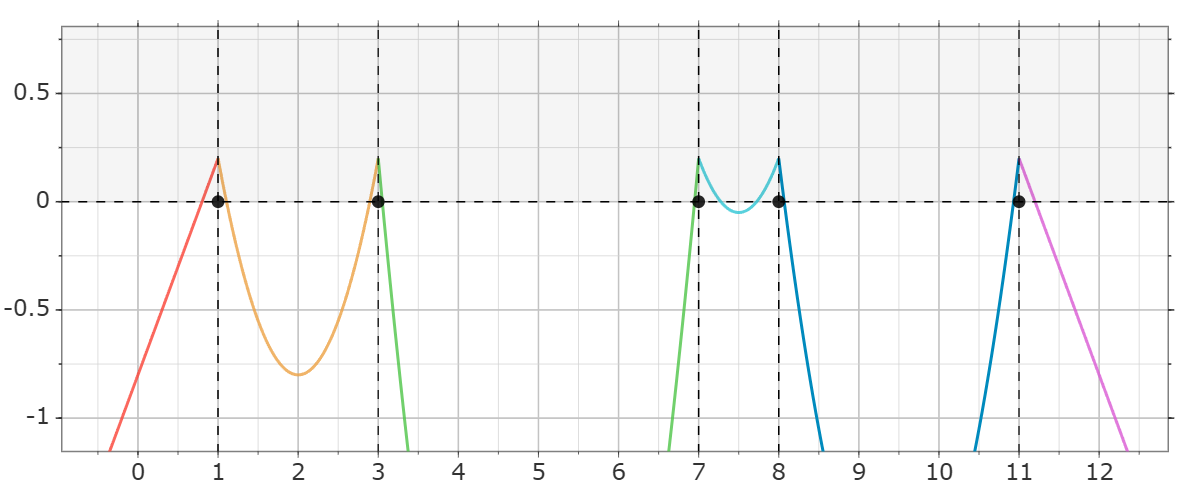
\includegraphics[width=0.8\textwidth]{psi.png}
  \caption{$\psi_i(w_i;\varepsilon)$ where $\varepsilon=0.2$ and $\mathcal{Q}_i=\{1,3,7,8,11\}$.}
  \includegraphics[width=0.8\textwidth]{psi2.png}
  \caption{The INT3 uniform quantization scheme, where $\varepsilon=0.2$ and $\mathcal{Q}_i=\{-4,-3,-2,-1,1,2,3,4\}$.}

\end{figure}

\newpage
\subsubsection{Part II. Asymptotic Convergence with Lipschitz Smoothness and Robbins-Monro Stepsizes}\hfill\\

\textbf{Significance.} This has largely improved the results of \texttt{ASkewSGD}'s convergence with incorporation of the mainstream stochastic analysis method. We can even generalize the constraint function $\psi$. This has left us with a class of candidate functions for selection (given that $\psi$ is Lipschitz-smooth).

\textit{Proof.} The \texttt{ASkewSGD} update is \[\mathbf{w}^{(k+1)}\gets\mathbf{w}^{(k)}+\gamma_k\hat{\mathbf{v}}^{(k)},\]
where $\hat{\mathbf{v}}^{(k)}=\mathbf{s}_{\varepsilon, \alpha}(\widehat{\nabla\ell}(\mathbf{w}^{(k)}),\mathbf{w}^{(k)})$, with the mean direction is $\mathbf{h}(\mathbf{w})=\mathbb{E}[\mathbf{s}_{\varepsilon, \alpha}(\widehat{\nabla\ell}(\mathbf{w}),\mathbf{w})|\mathbf{w}]$.

Consider the Stochastic Approximation (SA) Scheme, where we express the update as:
\[\mathbf{w}^{(k+1)}\gets\mathbf{w}^{(k)}+\gamma_k(\mathbf{h}(\mathbf{w}^{(k)})+\bm{\xi}^{(k)}),\]
where $\bm{\xi}^{(k)}=\hat{\mathbf{v}}^{(k)}-\mathbf{h}(\mathbf{w}^{(k)})$ is a martingale difference noise.

Define the Lyapunov function \[L(\mathbf{w})=\ell(\mathbf{w})+\frac{\alpha}{2}\sum_{i=1}^d [\min(0,\psi_i(\mathbf{w}))]^2.\]

Since $\ell\in C^1$, and the penalty term $[\min(0, \psi_i(w_i;\varepsilon))]^2$ is $C^1$ due to the piecewise $C^1$ structure of $\psi_i$ and the derivative continuity at boundaries, we know that $L$ is $C^1$.

Note that $\ell$ is also radially bounded (if $\ell$ is also coercive), with the gradient \[\nabla L(\mathbf{w})=\nabla \ell(\mathbf{w})+\mathbf{r}(\mathbf{w}), \text{where }r_i(\mathbf{w})=\begin{cases}0, &\psi_i(w_i;\varepsilon)> 0, \\
\alpha\psi_i(w_i;\varepsilon)\psi_i'(w_i;\varepsilon), &\psi_i(w_i;\varepsilon)\leq 0.
\end{cases}\] 

Moreover, $\mathbf{h}(\mathbf{w})=\mathbf{0}$ if and only if $\mathbf{w}\in\mathcal{Z}_\varepsilon$. 

We first prove the ``if'' direction. When $\mathbf{w}\in \mathcal{Z}_\varepsilon$ (which is a subset of $C_\varepsilon$), $\psi_i(w_i;\varepsilon)\geq 0$. If $\psi_i(w_i;\varepsilon)>0$, then $[\nabla\ell(\mathbf{w})]_i=0$. Otherwise, $\alpha\psi_i(w_i;\varepsilon)/\psi_i'(w_i;\varepsilon)=0$ and we just need to consider the case $-[\nabla\ell(\mathbf{w})]_i\cdot \psi_i'(w_i;\varepsilon)\geq  0$, this is impossible as $\text{sign}([\nabla\ell(\mathbf{w})]_i)=\text{sign}(\psi_i'(w_i;\varepsilon))$.

We then investigate the ``only-if'' direction. If $\psi_i(w_i;\varepsilon)>0$, we can make use of the fact that $[\nabla\ell(\mathbf{w})]_i=[h(\mathbf{w})]_i=0$. If $\psi_i(w_i;\varepsilon)< 0$ and $-[\nabla\ell(\mathbf{w})]_i\cdot \psi_i'(w_i;\varepsilon)\leq  \alpha \psi_i(w_i;\varepsilon)$, then $h(\mathbf{w})\neq 0$, which is a contradiction. This implies that $0=-[\nabla\ell(\mathbf{w})]_i\cdot \psi_i'(w_i;\varepsilon)\geq  \alpha \psi_i(w_i;\varepsilon)>0$, which is also impossible. If $\psi_i(w_i;\varepsilon)= 0$ and $-[\nabla\ell(\mathbf{w})]_i\cdot \psi_i'(w_i;\varepsilon)\leq  \alpha \psi_i(w_i;\varepsilon)=0$, then indeed we have $\text{sign}([\nabla\ell(\mathbf{w})]_i)=\text{sign}(\psi_i'(w_i;\varepsilon))$. Now, we are left with the conditions that takes $[h(\mathbf{w})]_i=-[\nabla\ell(\mathbf{w})]_i=0$ and $\psi_i(w_i;\varepsilon)\geq 0$, which is always satisfactory.

We need to prove the following claim.

\textit{Claim.} Almost surely, $\langle \nabla L(\mathbf{w}), \mathbf{h}(\mathbf{w})\rangle \leq -c\lVert \mathbf{h}(\mathbf{w})\rVert ^2$ for some $c>0$ when $\mathbf{h}(\mathbf{w})\neq 0$.

\begin{enumerate}[label=Case \arabic*., leftmargin=2.5cm]
\item If $w_i$ is strictly feasible, i.e. $\psi_i(\mathbf{w})> 0$, then $[\nabla L(\mathbf{w})]_i=[\nabla \ell(\mathbf{w})]_i$ and $[h(\mathbf{w})]_i=-[\nabla \ell(\mathbf{w})]_i$. Hence, \[[\nabla L(\mathbf{w})]_i [\mathbf{h}(\mathbf{w})]_i=-[\nabla \ell(\mathbf{w})]_i^2= -[\mathbf{h}(\mathbf{w})]_i ^2.\]
\item If $w_i$ is not strictly feasible, i.e. $\psi_i(\mathbf{w})\leq 0$, then $[\nabla L(\mathbf{w})]_i=[\nabla \ell(\mathbf{w})]_i+\alpha\psi_i(w_i;\varepsilon)\psi_i'(w_i;\varepsilon)$.
    \begin{enumerate}
        \item The gradient condition holds, i.e. $-[\nabla\ell(\mathbf{w})]_i\cdot\psi_i'(w_i;\varepsilon)\geq -\alpha \psi_i(w_i;\varepsilon)\geq 0$. Then, $[\mathbf{h}(\mathbf{w})]_i=-[\nabla \ell(\mathbf{w})]_i,$ \[\begin{aligned}[\nabla L(\mathbf{w})]_i\cdot [\mathbf{h}(\mathbf{w})]_i&=-[\nabla \ell(\mathbf{w})]_i^2-\alpha \psi_i(w_i;\varepsilon) \psi_i'(w_i;\varepsilon)\cdot [\nabla \ell(\mathbf{w})]_i\\
        &\leq-[\nabla\ell(\mathbf{w})]_i^2-\alpha^2\psi_i^2(w_i;\varepsilon)\leq -[\mathbf{h}(\mathbf{w})]_i ^2,\end{aligned}\] where \[-\alpha\psi_i(w_i;\varepsilon)\psi'_i(w_i;\varepsilon)\cdot[\nabla \ell(\mathbf{w})]_i\leq -\alpha \psi_i(w_i;\varepsilon)\cdot(\alpha\psi_i(w_i;\varepsilon))=-\alpha^2\psi_i(w_i;\varepsilon)^2.\]
        \item The gradient condition fails, i.e. $-[\nabla\ell(\mathbf{w})]_i\cdot\psi_i'(w_i;\varepsilon)< -\alpha \psi_i(w_i;\varepsilon)$. Then, $[\mathbf{h}(\mathbf{w})]_i=\text{clip}(-\alpha\psi_i(w_i;\varepsilon)/\psi_i'(w_i;\varepsilon), M_c)$. \\If $|[\mathbf{h}(\mathbf{w})]_i|\leq M_c$, then \[\begin{aligned}[\nabla L(\mathbf{w})]_i\cdot [\mathbf{h}(\mathbf{w})]_i&=([\nabla\ell(\mathbf{w})]_i+\alpha\psi_i(w_i;\varepsilon)\psi_i'(w_i;\varepsilon))\cdot (-\alpha\psi_i(w_i;\varepsilon)/\psi_i'(w_i;\varepsilon))\\
        & =-\alpha\frac{\psi_i(w_i;\varepsilon)\cdot[\nabla \ell(\mathbf{w})]_i}{\psi'_i(w_i;\varepsilon)}-\alpha^2\psi_i(w_i;\varepsilon)\\
        &<-\alpha^2\psi_i^2(w_i;\varepsilon)\left(\frac{1}{(\psi_i'(w_i;\varepsilon))^2}+1\right)\\
        &\leq -\left(\frac{\alpha\psi_i(w_i;\varepsilon)}{\psi_i'(w_i;\varepsilon)}\right)^2=-[\mathbf{h}(\mathbf{w})]_i^2. \end{aligned} \] Otherwise, assume that clipping is activated and $[\mathbf{h}(\mathbf{w})]_i=\varsigma M_c$, where $\varsigma=\text{sign}(-\alpha\psi_i(w_i;\varepsilon)/\psi_i'(w_i;\varepsilon))$. Since the case where $\psi_i'(w_i;\varepsilon)=0$ is measure-zero, then almost surely, \[\begin{aligned}[\nabla L(\mathbf{w})]_i\cdot [\mathbf{h}(\mathbf{w})]_i&=[\nabla L(\mathbf{w})]_i\cdot (-\alpha\psi_i(w_i;\varepsilon)/\psi_i'(w_i;\varepsilon))\cdot\frac{\varsigma M_c}{-\alpha\psi_i(w_i;\varepsilon)/\psi_i'(w_i;\varepsilon)}\\
        & \leq -(\alpha\psi_i(w_i;\varepsilon)/\psi_i'(w_i;\varepsilon))^2 \cdot \frac{\varsigma M_c}{-\alpha\psi_i(w_i;\varepsilon)/\psi_i'(w_i;\varepsilon)}\\
        &=(\alpha\psi_i(w_i;\varepsilon)/\psi_i'(w_i;\varepsilon)) \cdot \varsigma M_c\\
        &\leq -\varsigma^2M_c^2\quad\text{(since }|\alpha\psi_i(w_i;\varepsilon)/\psi_i'(w_i;\varepsilon)|\geq M_c\text{)}\\
        &= -M_c^2. \end{aligned} \]
    \end{enumerate}
\end{enumerate}

Thus, $L(\mathbf{w}(t))$ is almost surely non-increasing along trajectories.

Moreover, $L$ is radially unbounded, then $L(\mathbf{w}(t))$ converges to some $L^* \geq \inf L$ as $t \to \infty$.

Define the equilibrium set: \[
E = \left\{ \mathbf{w} : \frac{\text{d}}{\text{d}t}L(\mathbf{w}) = 0 \right\} \overset{\text{a.s.}}{=} \{ \mathbf{w} : h(\mathbf{w}) = 0 \} = \mathcal{Z}_\varepsilon
\] By LaSalle's Invariance Principle, the largest invariant set in $E$ is $\mathcal{Z}_\varepsilon$ (since $h(\mathbf{w}) = 0$ implies $\mathbf{w}(t)$ is constant). Hence,\[\lim_{t \to \infty} d(\mathbf{w}(t), Z_\varepsilon) = 0 \quad \text{a.s.}.\] For any $\epsilon > 0$, choose $\xi > 0$ such that \[\mathbf{w}(0) \in B_\xi(\mathcal{Z}_\varepsilon) \implies L(\mathbf{w}(0)) < \min_{\mathbf{w} \in \partial B_\epsilon(\mathcal{Z}_\varepsilon)} L(\mathbf{w}).\]
Since $L$ decreases along trajectories, $\mathbf{w}(t) \in B_\epsilon(\mathcal{Z}_\varepsilon)$ for all $t \geq 0$, and the set $Z_\varepsilon$ is almost surely globally asymptotically stable.

Via Kushner-Clark theorem, we verify that $\{\mathbf{w}^{(k)}\}$ bounded a.s., 
$\mathbb{E}[\bm{\xi}^{(k)} \mid \mathcal{F}_k] = 0$, $\mathbb{E}[\lVert \bm{\xi}^{(k)} \rVert^2 \mid \mathcal{F}_k] \leq \sigma^2$, $\sum \gamma_k = \infty, \quad \sum \gamma_k^2 < \infty$, and $Z_\varepsilon$ is almost surely globally asymptotically stable for ODE, and conclude that
\[
\lim_{k \to \infty} d(\mathbf{w}^{(k)}, \mathcal{Z}_\varepsilon) = 0 \quad \text{a.s.}.
\]\qed


% \marginpar{\small\textsf{\mbox{Jun 07, 2025}}}

% Consider the third statement. Define a filtration $\mathcal{F}_t\overset{\Delta}{=} \{\mathbf{x}_0, \bm{\xi}_0, \bm{\xi}_1, \ldots, \bm{\xi}_t-1\}$ for all $t\geq 1$ and $\mathcal{F}_0=\{\mathbf{x}_0\}$. From the previous part we have derived that

% \begin{align*}
% \mathbb{E}[\ell(\mathbf{w}^{(k+1)})|\mathcal{F}_k]
% &  \leq \ell(\mathbf{w}^{(k)}) - \sum\limits_{i\in\hat{S}_{1,\varepsilon}(\mathbf{w}^{(k)})\cup \hat{S}_{2,\varepsilon}(\mathbf{w}^{(k)})} [\nabla \ell(\mathbf{w}^{(k)})]_i^2 +\frac{L_\ell\gamma_k^2 \sigma^2}{2}+\gamma_k \mathbb{E}_{\mathbf{w}^{(k)}}\left[\sum\limits_{i\in \hat{S}_{3,\varepsilon}(\mathbf{w}^{(k)})\cup \hat{S}_{4,\varepsilon}(\mathbf{w}^{(k)})} 2\alpha\delta L_\ell\right]
% \end{align*}


\newpage
\section{Experimental Results}

\textbf{Two Moons Classification}. We train a five-layer MLP (shown as below) with a 2-dimensional input, and ReLU as activation function on the non-convex two moon classification task for $T=60$ epochs. Our dataset consists of $n=2000$ training samples (in batches of $200$ per iteration, points are colored in blue and red) and $m=500$ test samples (color in black and white), which is generated by \texttt{scikit-learn} library's \texttt{make\_moons} data generator. We have also added a random Gaussian noise with the variance of $\xi=0.1$ to offset the point from its original position. We apply the logistic loss function in this experiment. The learning rate $lr$ and the hyperparameter for ASkewSGD $\alpha$ are set to $0.2$ and $0.2$, respectively.
\begin{figure}[H]
  \centering
  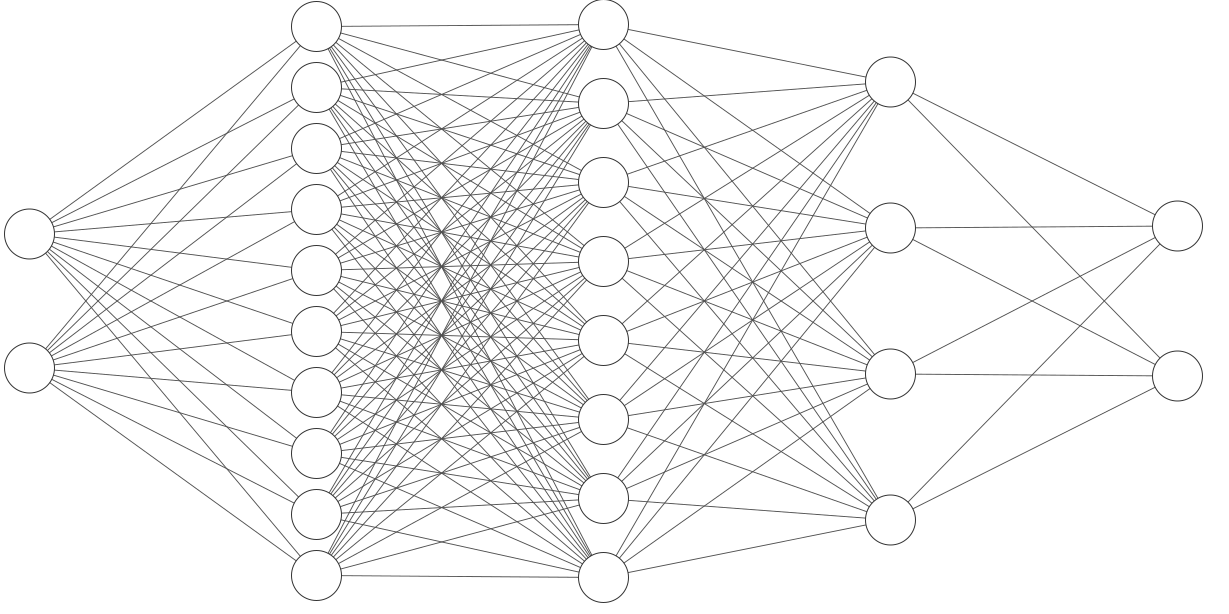
\includegraphics[width=0.6\linewidth]{nn.png}
\end{figure}

We compare SGD, BinaryConnect, and ASkewSGD to obtain the following results for the two moons classification problem. The first row shows the performance of different optimizers on the original net before quantization, and the second row depicts the quantized model with the quantization set $\mathcal{Q}=\{-1,+1\}$.

\begin{table}[H]
  \caption{Logistic loss after 60 epochs.} \label{Tb:tb1}
  \begin{center}
    \begin{tabular}{ccc}
      \hline
      Method                               & Loss             & Quantized Loss   \\ \hline
      Full Precision [W32/A32]             & 0.00002          & 0.59982          \\ \hline
      Deterministic BinaryConnect [W1/A32] & 0.57799          & 0.03260          \\
      \texttt{ASkewSGD} [W1/A32]           & \textbf{0.00367} & \textbf{0.00513} \\ \hline
    \end{tabular}
  \end{center}
\end{table}
\begin{figure}[H]
  \centering
  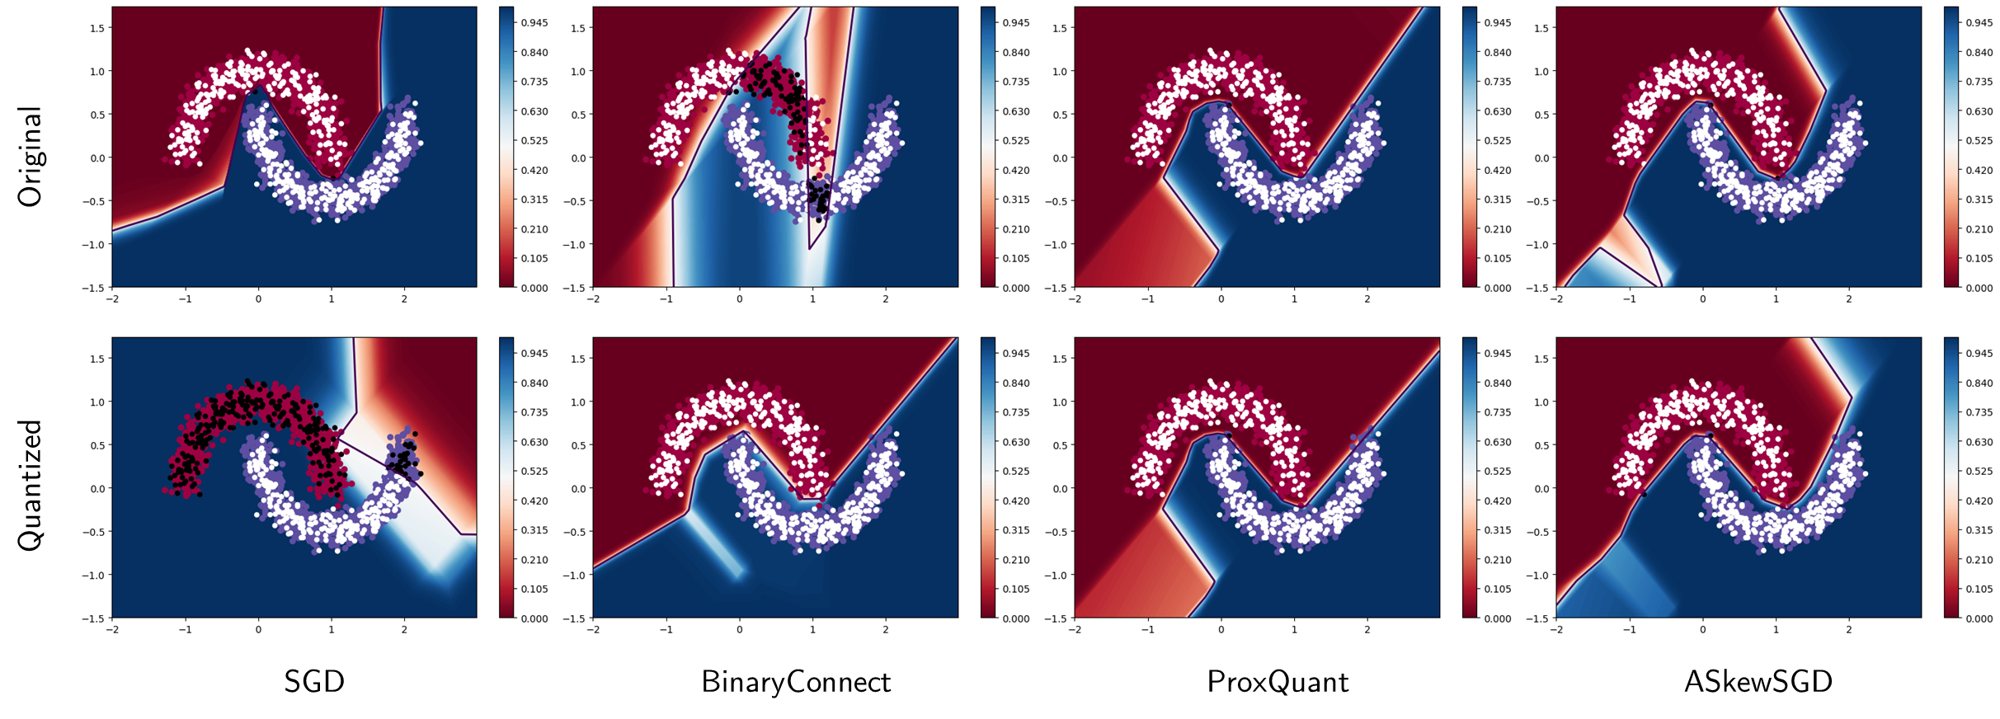
\includegraphics[width=0.7\linewidth]{twomoonstest.png}
\end{figure}
The original net has its contour completely perturbed by the weight quantization process. BinaryConnect is aware of the quantization scheme, thus generalizing well on the test set, but the original model is completely off from the groundtruth. ASkewSGD, on the other hand, has only a slight skew away from the sensible region, and the quantized model is still able to generalize well on the test set, which demonstrates the strength of this optimization method.

\newpage
\textbf{Computer Vision Task}. We train \texttt{ResNet-18} without bias and tunable parameters on the batch normalization layer on the CIFAR-10 dataset for $T=150$ epochs. The dataset consists of $n=50000$ training samples and $m=10000$ test samples. We apply the cross-entropy loss function in this experiment. We set the learning rate $lr$ and the hyperparameter for ASkewSGD $\alpha$ to $0.06$ and $0.2$, respectively. The quantization set $\mathcal{Q}$ is set to $\{-1,+1\}$.
\begin{figure}[H]
  \centering
  \includegraphics[width=0.9\linewidth]{CIFAR10_LO.png}
  \includegraphics[width=0.45\linewidth]{CIFAR10_AC.png}
  \includegraphics[width=0.45\linewidth]{CIFAR10_QA.png}
\end{figure}

\begin{table}[H]
  \caption{Performance of ResNet-18 on CIFAR10 after 60 epochs.} \label{Tb:tb1}
  \begin{center}
    \begin{tabular}{cccc}
      \hline
      Method                     & Accuracy & Loss    & Quantized Loss \\ \hline
      Full Precision [W32/A32]   & 88.91\%  & 0.04533 & 0.1            \\ \hline
      \texttt{ASkewSGD} [W1/A32] & 86.91\%  & 0.12337 & 0.8669         \\ \hline
    \end{tabular}
  \end{center}
\end{table}

It is worthwhile to note that the accuracy of the quantized model skyrocketed to $50\%$ only after running for 40 epochs, meaning that quantized models are sensitive to the accumulation of positional errors and the uncertain landscape of the loss function.

\newpage
\section{Improvements, Todos}
\begin{enumerate}[label=\text{[}\arabic*\text{]}]
  \item \texttt{ProxQuant}'s result is unlisted;
  \item Higher-bit experiments;
  \item Proofs...
\end{enumerate}

\newpage
\section{References}
\begin{enumerate}[label=\text{[}\arabic*\text{]}]
  \item \label{1}L. Leconte, S. Schechtman and E. Moulines. (2023). ASkewSGD: An Annealed Interval-Constrained Optimisation Method to Train Quantized Neural Networks. In \textit{Artificial Intelligence and Statistics 2023}, \textbf{206}:3644-3663.
  \item \label{2}T. Dockhorn, Y. Yu, E. Sari, M. Zolnouri, V. P. Nia. (2021). Demystifying and Generalizing BinaryConnect. In \textit{35th Conference on Neural Information Processing Systems (NeurIPS 2021)}. \url{arxiv.org/pdf/2110.13220}.
  \item \label{3}M. Muehlebach, M. I. Jordan. (2022). On Constraints in First-Order Optimization: A View from Non-Smooth Dynamical Systems. In \textit{Journal of Machine Learning Research}, \textbf{23}(256):1-47. \url{http://jmlr.org/papers/v23/21-0798.html}.
  \item \label{4}S. Ghadimi, G. Lan. (2013). Stochastic First- and Zeroth-Order Methods for Nonconvex Stochastic Programming. In \textit{SIAM Journal on Optimization}, \textbf{23}(4):2341-2368.

\end{enumerate}

\end{document}